\chapter{Optical Properties of Semiconductor}
\section{Maxwell Equations and Vector Potential}
The properties of electromagnetic fields in a medium are described by the four Maxwell equations. Apart from the electric field \( \mathbf{F} \), magnetic field \( \mathbf{B} \), and velocity of light, the effects of the material are represented by the dielectric constant \( \varepsilon \), permeability \( \mu \) (assumed \( \mu = \mu_0 \)), and electrical conductivity.
We start with the four Maxwell equations:
\begin{equation}
	\nabla \times \mathbf{F} + \frac{\partial \mathbf{B}}{\partial t} = 0, \quad
	\nabla \times \mathbf{H} - \frac{\partial \mathbf{D}}{\partial t} = \mathbf{J}, \quad
	\nabla \cdot \mathbf{D} = \rho, \quad
	\nabla \cdot \mathbf{B} = 0
\end{equation}
Here, \( \mathbf{D} = \varepsilon \mathbf{F} \), \( \mathbf{B} = \mu \mathbf{H} \), and \( \mathbf{J} \), \( \rho \) are current and charge densities, respectively.
In electron-photon interactions, it is convenient to use the scalar and vector potentials \( \phi \) and \( \mathbf{A} \), defined by:
\begin{equation}
	\mathbf{F} = -\frac{\partial \mathbf{A}}{\partial t} - \nabla \phi, \quad
	\mathbf{B} = \nabla \times \mathbf{A}
\end{equation}
These definitions automatically satisfy the first and fourth Maxwell equations. The potentials \( \phi \) and \( \mathbf{A} \) are not unique, and can be transformed using the gauge transformation:
\begin{equation}
	\mathbf{A}' = \mathbf{A} + \nabla \chi, \quad \phi' = \phi - \frac{\partial \chi}{\partial t}
\end{equation}
These transformations do not affect the physical fields \( \mathbf{F} \) and \( \mathbf{B} \).\\
Rewriting the second and third Maxwell equations in terms of \( \phi \) and \( \mathbf{A} \), we get:
\begin{equation}
	\frac{1}{\mu_0} \nabla \times (\nabla \times \mathbf{A}) + \varepsilon \frac{\partial^2 \mathbf{A}}{\partial t^2} + \varepsilon \nabla \left( \frac{\partial \phi}{\partial t} \right) = \mathbf{J}
\end{equation}
\begin{equation}
	\frac{\partial}{\partial t}(\nabla \cdot \mathbf{A}) + \nabla^2 \phi = -\frac{\rho}{\varepsilon}
\end{equation}
Using the identity:
\begin{equation}
	\nabla \times (\nabla \times \mathbf{A}) = \nabla (\nabla \cdot \mathbf{A}) - \nabla^2 \mathbf{A}
\end{equation}
We obtain:
\begin{equation}
	-\nabla^2 \mathbf{A} + \varepsilon \mu_0 \frac{\partial^2 \mathbf{A}}{\partial t^2} + \nabla \left( \nabla \cdot \mathbf{A} + \varepsilon \frac{\partial \phi}{\partial t} \right) = \mu_0 \mathbf{J}
\end{equation}
We now impose the Lorentz gauge condition:
\begin{equation}
	\nabla \cdot \mathbf{A} + \varepsilon \frac{\partial \phi}{\partial t} = 0
\end{equation}
This simplifies the Maxwell equations to:
\begin{equation}
	\nabla^2 \mathbf{A} - \varepsilon \mu_0 \frac{\partial^2 \mathbf{A}}{\partial t^2} = -\mu_0 \mathbf{J}, \quad
	\nabla^2 \phi - \varepsilon \mu_0 \frac{\partial^2 \phi}{\partial t^2} = -\frac{\rho}{\varepsilon}
\end{equation}
This form is especially useful for generalization to relativistic electrodynamics. In the **Coulomb (radiation) gauge**, where \( \mathbf{J} = 0 \) and \( \rho = 0 \), we may set \( \phi = 0 \) and \( \nabla \cdot \mathbf{A} = 0 \). The vector potential becomes a solution of the wave equation, typically:
\begin{equation}
	\mathbf{A}(\mathbf{r}, t) = \mathbf{A}_0 \left[ e^{i(\mathbf{k} \cdot \mathbf{r} - \omega t)} + \text{c.c.} \right]
\end{equation}
Where the wavevector \( \mathbf{k} \) and angular frequency \( \omega \) satisfy:
\begin{equation}
	|\mathbf{k}|^2 = \varepsilon \mu_0 \omega^2
\end{equation}
The corresponding electric and magnetic fields are:
\begin{equation}
	\mathbf{F} = -\frac{\partial \mathbf{A}}{\partial t} = 2\omega \mathbf{A}_0 \sin(\mathbf{k} \cdot \mathbf{r} - \omega t)
\end{equation}
\begin{equation}
	\mathbf{B} = \nabla \times \mathbf{A} = - 2\mathbf{k} \times \mathbf{A}_0 \sin(\mathbf{k} \cdot \mathbf{r} - \omega t)
\end{equation}
The Poynting vector representing the optical power is:
\begin{align}
	\mathbf{S} & = (\mathbf{F} \times \mathbf{H})                                                                       \\
	           & = \frac{4 v k^2}{\mu_0} \left| A_0 \right|^2 \sin^2(\mathbf{k} \cdot \mathbf{r} - \omega t) \, \hat{k}
\end{align}
The average power carried by the electromagnetic wave in the medium, where \( v = \frac{c}{\sqrt{\tilde{\epsilon}}} \) is the speed of light in the material and \( \hat{k} \) is the propagation direction unit vector, can be expressed as:
\begin{equation}
	\langle \mathbf{S} \rangle_{\text{time}} = \hat{k} \, \frac{2 v k^2 |\mathbf{A}_0|^2}{\mu_0}
\end{equation}
By rewriting the wave vector magnitude \( |\mathbf{k}| \) in terms of the angular frequency and the wave velocity, i.e.,
\begin{equation}
	|\mathbf{k}| = \frac{\omega}{v}
\end{equation}
we can substitute into the expression for the time-averaged Poynting vector to obtain:
\begin{equation}
	\langle \mathbf{S} \rangle_{\text{time}} = 2 v \epsilon \mu_0 \omega^2 |\mathbf{A}_0|^2 \hat{k}
\end{equation}
The energy stored per unit volume in the electromagnetic field can be related to the Poynting vector and the wave velocity as
\begin{equation}
	\left| \frac{S}{v} \right| = \frac{2 \epsilon \omega^2 |\mathbf{A}_0|^2}{c^2}
\end{equation}
Assuming a photon population of \( n_{\text{ph}} \), the energy density in a volume \( V \) becomes
\begin{equation}
	\frac{n_{\text{ph}} \hbar \omega}{V}
\end{equation}
Equating the two energy densities, we can isolate the amplitude of the vector potential:
\begin{equation}
	|\mathbf{A}_0|^2 = \frac{n_{\text{ph}} \hbar}{2 \epsilon \omega V}
\end{equation}
With these foundational relations established, we now consider wave propagation in a medium. By substituting \( \mathbf{J} = \sigma \mathbf{F} \) into Maxwell's equations and eliminating the magnetic field, we obtain the wave equation for the electric field:
\begin{equation}
	\nabla^2 \mathbf{F} = \epsilon \mu_0 \frac{\partial^2 \mathbf{F}}{\partial t^2} + \sigma \mu_0 \frac{\partial \mathbf{F}}{\partial t}
\end{equation}
This equation describes a damped wave. A general solution takes the form
\begin{equation}
	\mathbf{F} = \mathbf{F}_0 \exp \{ i(\mathbf{k} \cdot \mathbf{r} - \omega t) \}
\end{equation}
Substituting this into the wave equation yields the relation for the wavevector magnitude:
\begin{equation}
	-k^2 = -\epsilon \mu_0 \omega^2 - \sigma \mu_0 i \omega
\end{equation}
Or more compactly,
\begin{equation}
	k = \frac{\omega}{c} \left( \tilde{\epsilon} + \frac{\sigma \mu_0 i}{\omega} \right)^{1/2}
\end{equation}
Here, \( \tilde{\epsilon} \) represents the relative dielectric constant. In vacuum, where \( \sigma = 0 \) and \( \tilde{\epsilon} = 1 \), the wavevector simplifies to
\begin{equation}
	k = \frac{\omega}{c}
\end{equation}
Within a material, the propagation speed is affected by a complex refractive index \( n_r \), defined by
\begin{equation}
	n_r = \left( \tilde{\epsilon} + \frac{\sigma \mu_0 i}{\omega} \right)^{1/2}
\end{equation}
We can express \( n_r \) in terms of its real and imaginary parts as
\begin{equation}
	n_r = n_r' + i n_r''
\end{equation}
Substituting this into the expression for \( k \), we obtain
\begin{equation}
	k = \frac{n_r' \omega}{c} + i \frac{n_r'' \omega}{c}
\end{equation}
The electric field wave for propagation in the \( +z \) direction can be written as

\begin{equation}
	\mathbf{F} = \mathbf{F}_0 \exp\left\{ i\omega \left( \frac{n_r' z}{c} - t \right) \right\} \exp\left( \frac{-n_r'' \omega z}{c} \right)
\end{equation}
Here, the phase velocity is reduced by a factor \( n_r' \), making it \( c / n_r' \), and the wave amplitude decays exponentially as \( \exp(-2\pi n_r'' / n_r') \) per wavelength. This decay in amplitude is a result of absorption of the electromagnetic energy.\\
The absorption coefficient \( \alpha \), which characterizes the intensity loss, is given by
\begin{equation}
	\alpha = \frac{2 n_r'' \omega}{c}
\end{equation}
In the special case where there is no absorption, the real part of the refractive index \( n_r' \) equals the total refractive index \( n_r \), and \( n_r'' = 0 \).\\
The absorption coefficient is measurable and provides direct information about the imaginary component \( n_r'' \) of the refractive index.\\
The interaction of the medium with the electromagnetic field is fully described by a complex dielectric constant or equivalently a complex refractive index. The real and imaginary parts of the dielectric constant \( \tilde{\epsilon} \) are related to the refractive index components as follows:
\begin{equation}
	\tilde{\epsilon}_1 = n_r'^2 - n_r''^2, \qquad
	\tilde{\epsilon}_2 = 2 n_r' n_r''
\end{equation}
These expressions relate the real (\( \tilde{\epsilon}_1 \)) and imaginary (\( \tilde{\epsilon}_2 \)) parts of the relative permittivity to the components of the complex refractive index.\\
A very significant relationship exists between the real and imaginary parts of the refractive index based on causality—this is known as the Kramers–Kronig relation. It connects the frequency-dependent refractive index to the absorption coefficient via
\begin{equation}
	n(\omega_0) - 1 = \frac{c}{\pi} \mathcal{P} \int_0^\infty \frac{\alpha(\omega)}{\omega^2 - \omega_0^2} \, d\omega
\end{equation}
This formulation is powerful as it enables the calculation of the refractive index if the absorption coefficient is known. In cases where the absorption spectrum varies under external influences (e.g., electric fields), changes in the refractive index can be predicted accordingly.


\section{Electrons in Electromagnetic Field}
Electrons, possessing a negative charge, interact with electric and magnetic fields originating from electromagnetic radiation. The electric field exerts a force equal to the product of the charge and the field itself, whereas the magnetic field contributes through the Lorentz force, which involves the cross product between the electron's velocity and the magnetic field.\\
This interaction energy defines the interaction Hamiltonian, which plays a central role in electron scattering processes. The total Hamiltonian for a charge \( e \) in the presence of an electromagnetic field is
\begin{equation}
	H = \frac{1}{2m_0} (\mathbf{p} - e \mathbf{A})^2 + e \phi + V(\mathbf{r})
\end{equation}
Expanding the square and rearranging terms:
\begin{equation}
	H = \frac{\mathbf{p}^2}{2m_0} - \frac{e}{2m_0} (\mathbf{p} \cdot \mathbf{A} + \mathbf{A} \cdot \mathbf{p}) + \frac{e^2}{2m_0} \mathbf{A}^2 + e \phi + V(\mathbf{r})
\end{equation}
In this expression, \( \mathbf{A} \) denotes the vector potential and \( V(\mathbf{r}) \) represents any potential due to the crystal lattice.\\
Within the framework of quantum mechanics, the momentum operator \( \mathbf{p} \) is defined differentially. Therefore, the operator form of \( \mathbf{p} \cdot \mathbf{A} \) becomes
\begin{equation}
	\frac{e}{2m_0} \mathbf{p} \cdot \mathbf{A} = \frac{e}{2m_0} \mathbf{A} \cdot \mathbf{p} - \frac{i e \hbar}{2m_0} \nabla \cdot \mathbf{A}
\end{equation}
Substituting this result into the Hamiltonian yields
\begin{equation}
	H = \frac{\mathbf{p}^2}{2m_0} - \frac{e}{m_0} \mathbf{A} \cdot \mathbf{p} + \frac{i e \hbar}{2m_0} \nabla \cdot \mathbf{A} + \frac{e^2}{2m_0} \mathbf{A}^2 + e \phi + V(\mathbf{r})
\end{equation}
To analyze the influence of electromagnetic radiation on an electron, we apply perturbation theory. In the quantum mechanical description of radiation, the electromagnetic field is represented using creation and annihilation operators, akin to those used in harmonic oscillator problems—similar to the formalism previously applied to phonon interactions.\\
The time-dependent Schrödinger equation describing this system is then:
\begin{equation}
	i \hbar \frac{\partial \psi}{\partial t} = \left[
		- \frac{\hbar^2}{2m_0} \nabla^2
		+ \frac{i e \hbar}{m_0 c} \mathbf{A} \cdot \nabla
		+ \frac{i e \hbar}{2 m_0} (\nabla \cdot \mathbf{A})
		+ \frac{e^2}{2 m_0} \mathbf{A}^2
		+ e \phi + V(\mathbf{r})
		\right] \psi
\end{equation}
We adopt the radiation gauge, where \( \nabla \cdot \mathbf{A} = \phi = 0 \), and use time-dependent perturbation theory to compute scattering rates using Fermi’s golden rule. Assuming the optical power is modest, the vector potential \( \mathbf{A} \) remains small, so we can estimate:
\begin{equation}
	\left| \frac{i e \hbar}{m_0} \mathbf{A} \cdot \nabla \right| : \left| \frac{\hbar^2}{2m_0} \nabla^2 \right| \approx \left| \frac{e^2 A^2}{2m_0^2} \right| : \left| \frac{i e \hbar}{m_0} \mathbf{A} \cdot \nabla \right| \approx \frac{eA}{p}
\end{equation}
For an optical intensity of 1 W/cm\(^2\), the corresponding photon density at 1 eV energy is approximately \( 10^9 \,\text{cm}^{-3} \). With an electron velocity of \( 10^6 \,\text{cm/s} \), we find:
\begin{equation}
	\frac{eA}{p} \sim 10^{-5}
\end{equation}
This implies that even for a beam as intense as 1 MW/cm\(^2\), the quantity \( eA/p \) remains sufficiently small for perturbation theory to be applicable. Therefore, we will only consider terms linear in \( \mathbf{A} \).\\
The time-dependent Schrödinger equation now simplifies to:
\begin{equation}
	i \hbar \frac{\partial \psi}{\partial t} = (H_0 + H') \psi
\end{equation}
where the unperturbed Hamiltonian is:
\begin{equation}
	H_0 = -\frac{\hbar^2}{2m_0} \nabla^2 + V(\mathbf{r})
\end{equation}
and the perturbation is given by:
\begin{equation}
	H' = \frac{i e \hbar}{m_0} \mathbf{A} \cdot \nabla
\end{equation}
\begin{center}
	\begin{minipage}{0.8\textwidth}
		\centering
		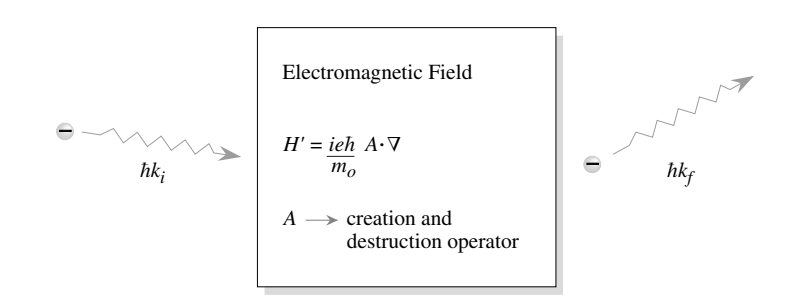
\includegraphics[width=\textwidth]{img/Scattering.png}
		\\[0.5em]
		\refstepcounter{figure}
		\textbf{Figure~\thefigure.} Schematic of the scattering process of an electron by the electromagnetic field.
		\label{fig:Scattering}
	\end{minipage}
\end{center}
The scattering process arises from this perturbation, where the electromagnetic field induces transitions in the electron states. In the second quantization framework, \( \mathbf{A} \) is quantized using photon creation and annihilation operators \( b^\dagger \) and \( b \), analogous to the harmonic oscillator treatment.\\
According to Fermi’s golden rule, the transition rate from an initial state \( |i\rangle \) to a final state \( |f\rangle \) is:
\begin{equation}
	W(i) = \frac{2\pi}{\hbar} \sum_f \left| \langle f | H' | i \rangle \right|^2 \delta \left( E_f - E_i \mp \hbar \omega \right)
\end{equation}
Here, the upper sign corresponds to photon absorption and the lower sign to emission.\\
The initial and final states are described by the electron's momentum and the photon number.

In the case of photon \textbf{absorption}, the states are:
\begin{align*}
	|i\rangle & = |k_i, n_{\text{ph}} \rangle     \\
	|f\rangle & = |k_f, n_{\text{ph}} - 1 \rangle
\end{align*}
\textbf{Emission:}
\begin{align*}
	|i\rangle & = |k_i, n_{\text{ph}}\rangle     \\
	|f\rangle & = |k_f, n_{\text{ph}} + 1\rangle
\end{align*}
Here, \(k_i\) and \(k_f\) denote the initial and final wavevectors of the electron, respectively, and \(n_{\text{ph}}\) is the initial photon occupation number. The vector potential \(A_0\) is defined as:
\begin{equation}
	A_0 = \sqrt{\frac{\hbar}{2 \omega \epsilon V}} \left(b^\dagger + b\right)
\end{equation}
In this expression, \(b^\dagger\) and \(b\) are the photon creation and annihilation operators. This form is chosen to be consistent with the magnitude \(|A_0|^2\) used previously.\\
When calculating matrix elements, we consider the photon operators separately. Let \( \mathbf{a} \) represent the polarization unit vector. Focusing on the matrix element due to the photon part only:
\textbf{Absorption:}
\begin{align*}
	\langle f | \mathbf{A} \cdot \nabla | i \rangle & \Rightarrow
	\sqrt{\frac{\hbar}{2 \omega \epsilon}} \left\langle k_f, n_{\text{ph}} - 1 \middle| \left(b^\dagger + b\right) \mathbf{a} \cdot \nabla \middle| k_i, n_{\text{ph}} \right\rangle             \\
	                                                & = \sqrt{\frac{\hbar}{2 \omega \epsilon}} \sqrt{n_{\text{ph}}} \left\langle k_f \middle| \mathbf{a} \cdot \nabla \middle| k_i \right\rangle
\end{align*}
\textbf{Emission:}
\begin{align*}
	\langle f | \mathbf{A} \cdot \nabla | i \rangle & \Rightarrow
	\sqrt{\frac{\hbar}{2 \omega \epsilon}} \left\langle k_f, n_{\text{ph}} + 1 \middle| \left(b^\dagger + b\right) \mathbf{a} \cdot \nabla \middle| k_i, n_{\text{ph}} \right\rangle                 \\
	                                                & = \sqrt{\frac{\hbar}{2 \omega \epsilon}} \sqrt{n_{\text{ph}} + 1} \left\langle k_f \middle| \mathbf{a} \cdot \nabla \middle| k_i \right\rangle
\end{align*}
It is crucial to notice the difference in prefactors: \( \sqrt{n_{\text{ph}}} \) appears for absorption, while \( \sqrt{n_{\text{ph}} + 1} \) appears for emission. This distinction will play a significant role in later discussions.
To proceed with calculating the rate for photon absorption—where a photon of energy \(\hbar \omega\) and momentum \(\hbar k_{\text{ph}}\) is absorbed by an electron—we will need to sum over all possible electron states which can allow such a process to occur.\\
\begin{center}
	\begin{minipage}{0.5\textwidth}
		\centering
		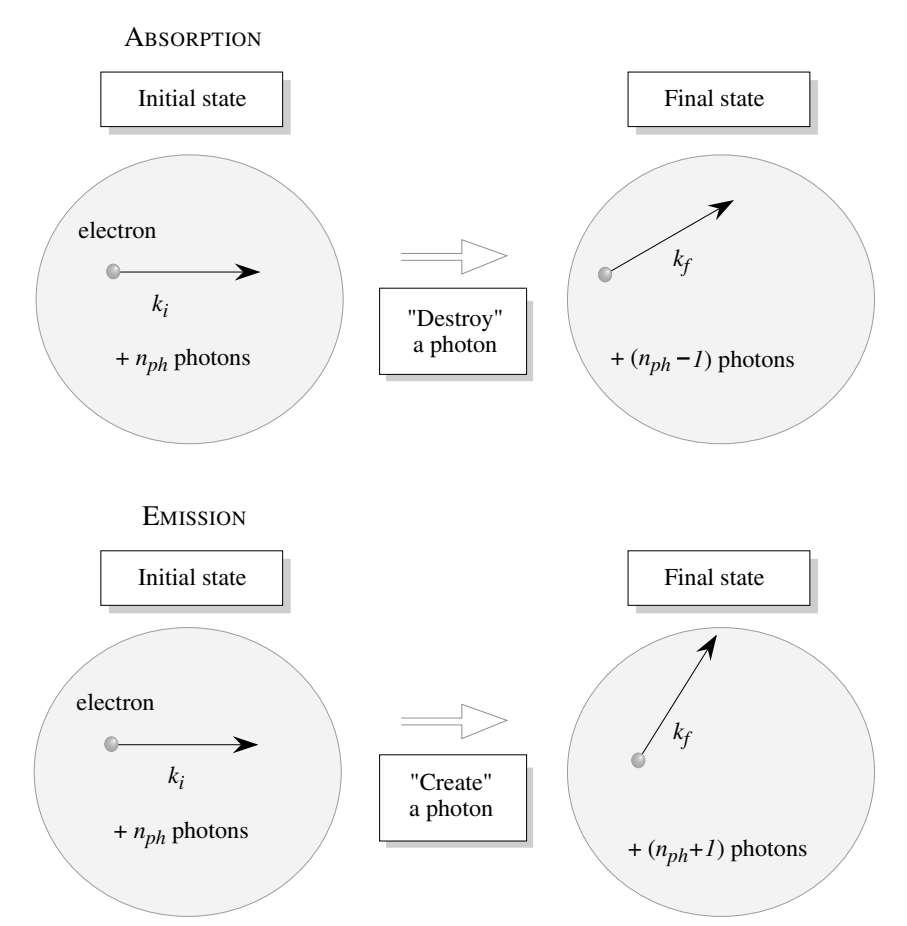
\includegraphics[width=\textwidth]{img/Abs&emiss.png}
		\\[0.5em]
		\refstepcounter{figure}
		\textbf{Figure~\thefigure.} (a) Schematic of a photon absorption process, where a photon is annihilated and the electron’s energy and momentum change.
		(b) Photon emission process, where a photon is generated as the electron transitions to a lower energy state.
		\label{fig:Abs&emiss}
	\end{minipage}
\end{center}
The process of photon absorption involves the transfer of photon energy \(\hbar \omega\) to an electron. To compute the full scattering rate, we integrate over the final electron density of states:
\begin{equation}
	W_{\text{abs}} = \frac{2\pi}{\hbar} \frac{e^2}{m_0^2} \left( \frac{\hbar n_{\text{ph}}}{2 \omega \epsilon} \right) \sum_{\text{final states}} \left| \int \psi_f^* (\mathbf{a} \cdot \mathbf{p}) e^{i \mathbf{k}_{\text{ph}} \cdot \mathbf{r}} \psi_i \, d^3r \right|^2 \delta(E_i - E_f + \hbar \omega)
\end{equation}
This expression includes a sum over all possible electronic final states for photon absorption, ensuring energy conservation. Alternatively, one might be interested in electron scattering from an initial state with momentum \(k_i\) to a final state with momentum \(k_f\), summing instead over photon states that enable this transition.\\
For photon emission, where an electron in state \(\hbar k_i\) emits a photon and transitions to \(\hbar k_f\), the corresponding rate is:
\begin{equation}
	W_{\text{em}} = \frac{2\pi}{\hbar} \frac{e^2}{m_0^2} \left( \frac{\hbar(n_{\text{ph}} + 1)}{2 \omega \epsilon} \right) \sum_{\text{final states}} \left| \int \psi_f^* (\mathbf{a} \cdot \mathbf{p}) e^{-i \mathbf{k}_{\text{ph}} \cdot \mathbf{r}} \psi_i \, d^3r \right|^2 \delta(E_i - E_f - \hbar \omega)
\end{equation}
This emission rate can be broken into two components: one for stimulated emission and one for spontaneous emission:
\begin{equation}
	W_{\text{em}} = W_{\text{st}} + W_{\text{spon}}
\end{equation}
where
\begin{equation}
	W_{\text{st}} = \frac{2\pi}{\hbar} \frac{e^2}{m_0^2} \frac{\hbar n_{\text{ph}}}{2 \omega \epsilon} \sum_{\text{final states}} \left| \int \psi_f^* e^{-i \mathbf{k}_{\text{ph}} \cdot \mathbf{r}} (\mathbf{a} \cdot \mathbf{p}) \psi_i \, d^3r \right|^2 \delta(E_i - E_f - \hbar \omega)
\end{equation}
\begin{equation}
	W_{\text{spon}} = \frac{2\pi}{\hbar} \frac{e^2}{m_0^2} \frac{\hbar}{2 \omega \epsilon} \sum_{\text{final states}} \left| \int \psi_f^* e^{-i \mathbf{k}_{\text{ph}} \cdot \mathbf{r}} \psi_i \, d^3r \right|^2 \delta(E_i - E_f - \hbar \omega)
\end{equation}
\textit{Stimulated emission} arises from the presence of photons already in the system, and the emitted photons are phase coherent with the initial ones. \textit{Spontaneous emission}, on the other hand, originates from quantum vacuum fluctuations (\(n_{\text{ph}} = 0\)) and results in photons that are phase-incoherent.\\
This distinction is fundamental in understanding the operational differences between devices such as LEDs and laser diodes.\\
When examining semiconductor states, we observe that the photon momentum \(\hbar k_{\text{ph}}\), for typical photon energies between 0.1 and 2.0 eV, is much smaller than the electron momentum. Therefore, momentum conservation requires that:
\begin{equation}
	k_i = k_f
\end{equation}
In first-order perturbation theory, transitions triggered by photon absorption or emission are represented as "vertical" processes in the energy–momentum (\(E\)-\(k\)) diagram. This is particularly evident in interband transitions. When the photon momentum \(k_{\text{ph}}\) is small enough to be neglected, the approximation is referred to as the dipole approximation. Under this approximation, the momentum matrix element (the integral within the absolute value bars in the relevant transition rate equations) simplifies significantly. We denote this matrix element as \(p_{if}\).\\
Let us now consider the case where both the initial and final states follow the Bloch form. In the dipole approximation, the momentum matrix element becomes:
\begin{equation}
	p_{if} = -i\hbar \int \psi^*_{\mathbf{k}_f \ell'} \, \nabla \psi_{\mathbf{k}_i \ell} \, d^3 r
\end{equation}
We define the initial and final Bloch states as follows:
\[
	\begin{aligned}
		|i\rangle & = \psi_{\mathbf{k}_i, \ell} = e^{i \mathbf{k}_i \cdot \mathbf{r}} u_{\mathbf{k}_i \ell},   \\
		|f\rangle & = \psi_{\mathbf{k}_f, \ell'} = e^{i \mathbf{k}_f \cdot \mathbf{r}} u_{\mathbf{k}_f \ell'},
	\end{aligned}
\]
where \( u_{\mathbf{k} \ell} \) denotes the cell-periodic part of the Bloch wavefunction, and \(\ell\), \(\ell'\) are band indices.\\
By applying the gradient operator to the initial state, the momentum matrix element simplifies into the following form:
\begin{equation}
	p_{if} = \hbar \mathbf{k}_i \int \psi^*_{\mathbf{k}_f \ell'} \psi_{\mathbf{k}_i \ell} \, d^3 r
	- i\hbar \int u^*_{\mathbf{k}_f \ell'} \left( \nabla u_{\mathbf{k}_i \ell} \right)
	e^{i(\mathbf{k}_i - \mathbf{k}_f) \cdot \mathbf{r}} \, d^3 r
\end{equation}
\begin{figure}[H]
	\centering
	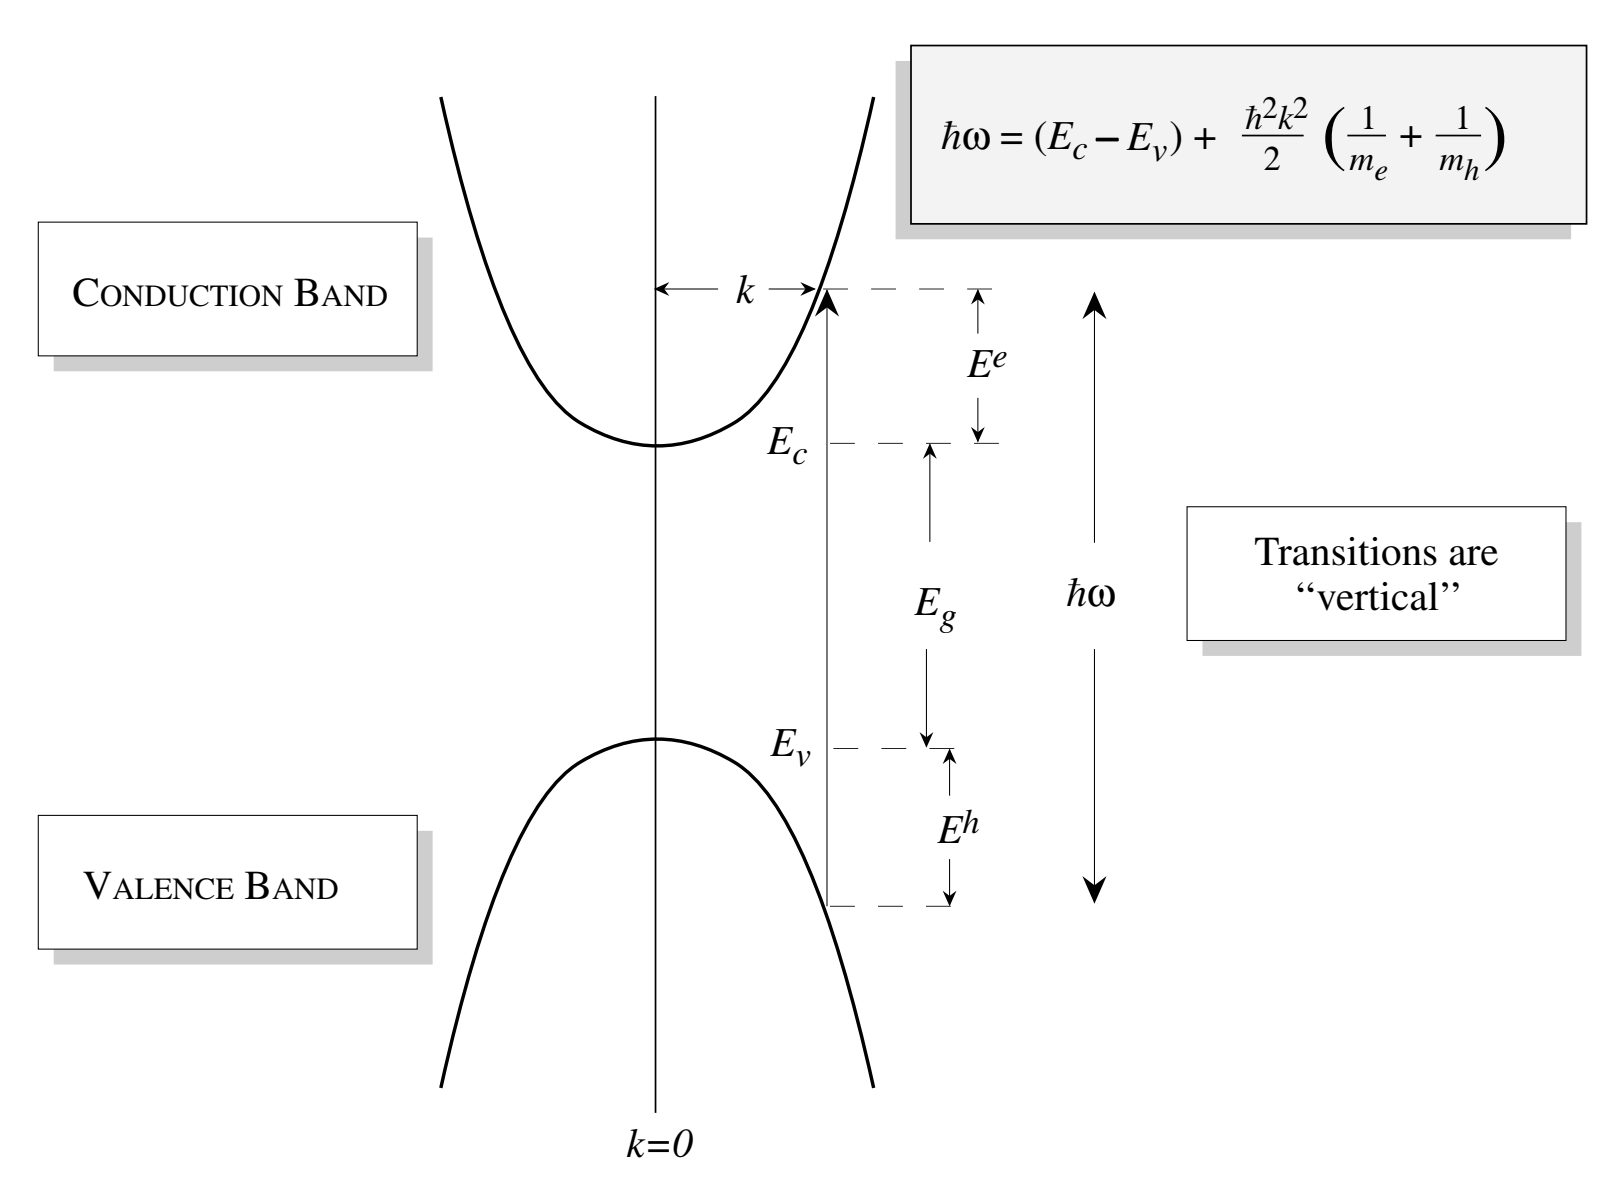
\includegraphics[width=0.8\textwidth]{img/transitions.png}
	\caption{Electron and hole energy levels at vertical \(\mathbf{k}\)-values. The transition energies are set by the photon energy and the effective masses of the carriers. Due to the negligible photon momentum, these transitions occur vertically in \(\mathbf{k}\)-space.
	}
	\label{fig:transitions}
\end{figure}



\section{Interband Transitions}
\subsection{Interband Transitions in Bulk Semiconductors}
We now examine the selection rules governing band-to-band transitions in direct-gap semiconductors. For instance, zincblende materials such as GaAs, InAs, and InP. We use the properties of the conduction and valence band central cell functions to simplify the momentum matrix elements. The first term in the momentum matrix expression vanishes due to orthogonality of Bloch states, and we are left with a nonzero contribution only when:
\begin{equation}
	\mathbf{k}_i - \mathbf{k}_f = 0
\end{equation}
This condition implies that the transitions are “vertical” in \( \mathbf{k} \)-space, and the matrix element for interband transitions reduces to:
\begin{equation}
	\langle u_{c\mathbf{k}} | \mathbf{p}_a | u_{v\mathbf{k}} \rangle
\end{equation}
where \( u_{c\mathbf{k}} \) and \( u_{v\mathbf{k}} \) represent the central cell wavefunctions for the conduction and valence bands, respectively.\\
Near the band edge, we approximate \( u_{c\mathbf{k}} \) and \( u_{v\mathbf{k}} \) by their values at the Brillouin zone center. Specifically:
\begin{equation}
	u_{c0} = |s\rangle
\end{equation}
where \( |s\rangle \) denotes a spherically symmetric conduction band state.\\
The valence band states are given by:
\begin{align}
	\text{\textbf{Heavy Hole states:}} \quad |3/2, 3/2\rangle & = \frac{-1}{\sqrt{2}} (|p_x\rangle + i |p_y\rangle) |\uparrow\rangle                                                   \\
	|3/2, -3/2\rangle                                         & = \frac{1}{\sqrt{2}} (|p_x\rangle - i |p_y\rangle) |\downarrow\rangle                                                  \\
	\text{\textbf{Light Hole states:}}\quad |3/2, 1/2\rangle  & = \frac{-1}{\sqrt{6}} \left[ (|p_x\rangle + i |p_y\rangle) |\downarrow\rangle - 2 |p_z\rangle |\uparrow\rangle \right] \\
	|3/2, -1/2\rangle                                         & = \frac{1}{\sqrt{6}} \left[ (|p_x\rangle - i |p_y\rangle) |\uparrow\rangle + 2 |p_z\rangle |\downarrow\rangle \right]
\end{align}
By symmetry, only matrix elements of the form:
\begin{equation}
	\langle p_x | p_x | s \rangle = \langle p_y | p_y | s \rangle = \langle p_z | p_z | s \rangle = p_{cv}
\end{equation}
are nonzero. Hence, for band-to-band transitions, the allowed nonzero matrix elements are:
\begin{align}
	\langle \text{HH} | p_x | s \rangle & = \langle \text{HH} | p_y | s \rangle = \frac{1}{\sqrt{2}} \langle p_x | p_x | s \rangle \\
	\langle \text{LH} | p_x | s \rangle & = \langle \text{LH} | p_y | s \rangle = \frac{1}{\sqrt{6}} \langle p_x | p_x | s \rangle
\end{align}
Additionally, we have:
\begin{equation}
	\langle \text{LH} | p_z | s \rangle = \frac{2}{\sqrt{6}} \langle p_x | p_x | s \rangle = \frac{2}{\sqrt{6}} p_{cv}
\end{equation}
It is worth noting that:
\begin{equation}
	\langle \text{HH} | p_z | s \rangle = 0
\end{equation}
It is useful to examine how the squared matrix elements depend on the polarization direction of incident light. In quantum wells, this effect is enhanced due to the heavy-hole (HH) and light-hole (LH) splitting.

\textbf{z-polarized light}:
\begin{align*}
	\text{HH} \rightarrow \text{c-band:} & \quad \text{No coupling}                                                  \\
	\text{LH} \rightarrow \text{c-band:} & \quad |\mathbf{p}_{if}|^2 = \frac{2}{3} |\langle p_x | p_x | s \rangle|^2
\end{align*}
\textbf{x-polarized light}:
\begin{align}
	\text{HH} \rightarrow \text{c-band:} & \quad |\mathbf{p}_{if}|^2 = \frac{1}{2} |\langle p_x | p_x | s \rangle|^2 \\
	\text{LH} \rightarrow \text{c-band:} & \quad |\mathbf{p}_{if}|^2 = \frac{1}{6} |\langle p_x | p_x | s \rangle|^2
\end{align}
\textbf{y-polarized light}:
\begin{align*}
	\text{HH} \rightarrow \text{c-band:} & \quad |\mathbf{p}_{if}|^2 = \frac{1}{2} |\langle p_x | p_x | s \rangle|^2 \\
	\text{LH} \rightarrow \text{c-band:} & \quad |\mathbf{p}_{if}|^2 = \frac{1}{6} |\langle p_x | p_x | s \rangle|^2
\end{align*}
This shows that z-polarized light does not interact with heavy-hole states. At \( \mathbf{k} = 0 \), states are pure; further from the zone center, HH and LH states mix. x- and y-polarized light couple more strongly with HH than LH states. This selection rule behavior is crucial in designing lasers and photodetectors.\\
To simplify notation, we define:
\begin{equation}
	E_p = \frac{2}{m_0} |\langle p_x | p_x | s \rangle|^2
\end{equation}
For direct transitions using the parabolic band approximation, we have:
\begin{equation}
	\hbar \omega - E_g = \frac{\hbar^2 k^2}{2} \left( \frac{1}{m_e^*} + \frac{1}{m_h^*} \right) = \frac{\hbar^2 k^2}{2 m_r^*}
\end{equation}
Here, \( m_r^* \) is the reduced mass of the electron-hole pair.
The reduced joint density of states is given by:
\begin{equation}
	N_{cv}(\hbar \omega) = \frac{\sqrt{2} (m_r^*)^{3/2} (\hbar \omega - E_g)^{1/2}}{\pi^2 \hbar^3}
\end{equation}
Combining this with the previous expression for absorption rate, we get:
\begin{equation}
	W_{abs} = \frac{\pi e^2 \hbar n_{ph}}{\epsilon m_0^2 \omega} |\mathbf{a} \cdot \mathbf{p}|_{cv}^2 N_{cv}(\hbar \omega)
\end{equation}
In bulk semiconductors, for unpolarized light, the absorption rate becomes (from previous expressions):
\begin{equation}
	W_{\text{abs}} = \frac{\pi e^2 \hbar n_{ph}}{2 \epsilon m_0 \hbar \omega} \left( \frac{2 p_{cv}^2}{m_0} \right) \frac{2}{3} N_{cv}(\hbar \omega)
\end{equation}
Before comparing absorption and recombination in bulk and quantum wells, we briefly relate the absorption rate to the absorption coefficient. Considering photons traveling along the \(x\)-axis, we write the photon density continuity equation as:
\begin{equation}
	\frac{dn_{ph}}{dt} = \left. \frac{\partial n_{ph}}{\partial t} \right|_{\text{vol}} + \frac{\partial (v n_{ph})}{\partial x}
\end{equation}
The first term on the right-hand side is due to absorption, and the second to spatial variation in photon current. In steady-state, the photon density can be modeled as:
\begin{equation}
	n_{ph}(x) = n_0 \exp(-\alpha x)
\end{equation}
which defines the absorption coefficient \(\alpha\). Also, since:
\begin{equation}
	\frac{\partial n_{ph}}{\partial t} = W_{\text{abs}}
\end{equation}
In steady-state we have:
\begin{equation}
	W_{\text{abs}} = \alpha v n_{ph}
\end{equation}
Solving for \(\alpha\), the absorption coefficient is given by:
\begin{equation}
	\alpha = \frac{W_{\text{abs}}}{v n_{ph}}
\end{equation}
\begin{center}
	\begin{minipage}{0.5\textwidth}
		\centering
		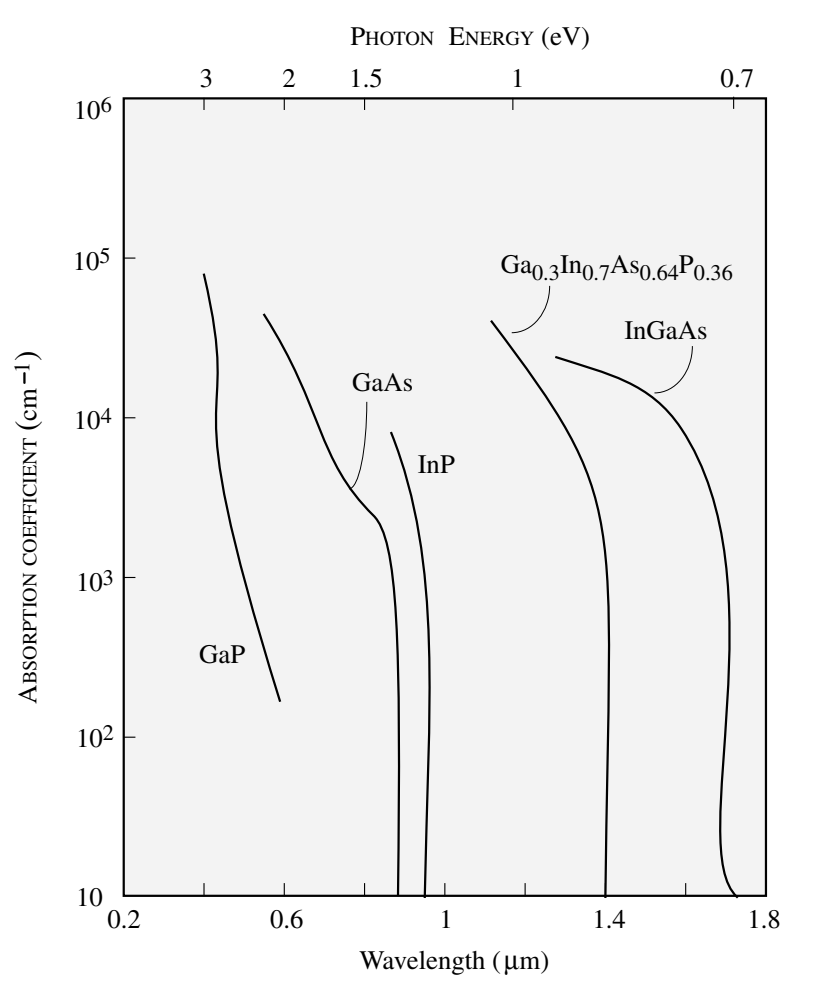
\includegraphics[width=\textwidth]{img/Abs_coeff.png}
		\\[0.5em]
		\refstepcounter{figure}
		\textbf{Figure~\thefigure.} Absorption coefficient for several semiconductors.
		\label{fig:Abs_coeff}
	\end{minipage}
\end{center}
For the total emission rate, the expression becomes:
\begin{equation}
	W_{\text{em}} = \frac{\pi e^2 \hbar}{m_0^2 \hbar \omega \epsilon} \left( n_{ph} + 1 \right) \left| \mathbf{a} \cdot \mathbf{p}_{if} \right|^2 \rho_a(\hbar \omega)
\end{equation}
where \(\rho_a\) is the photon density of states for the polarization vector \(\mathbf{a}\). The total photon density of states, accounting for two transverse polarization modes per \(\mathbf{k}\)-value, is given by:
\begin{equation}
	\rho(\hbar \omega) = \frac{2 \omega^2}{2 \pi^2 \hbar v^3}
\end{equation}
This expression applies to photons emitted in three-dimensional space. In the case where \(n_{ph} = 0\), the emission rate reduces to the spontaneous emission rate \(W_{\text{spon}}\). Its inverse defines the electron-hole recombination time \(\tau_o\). The quantity \(\tau_o\) represents the average time required for an electron in a given state \(\mathbf{k}\) to recombine with an available hole in the same state.



\subsection{Interband Transitions in Quantum Wells}
The formalism developed so far can be straightforwardly adapted to quantum well structures. In this context, the central cell functions are mostly unaffected by the confining potential. The main differences are the modified wavefunctions—confined in the well—and the step-like density of states characteristic of 2D parabolic bands.\\
The electron and hole wavefunctions in the quantum well, using the envelope function approximation, are written as:
\begin{equation}
	\psi^n_c = \frac{1}{\sqrt{AW}} e^{i \mathbf{k}_\rho \cdot \mathbf{\rho}}\, g_c^n(z)\, u_{c \mathbf{k}_c}^n, \quad
	\psi^m_v = \frac{1}{\sqrt{AW}} e^{i \mathbf{k}_\rho \cdot \mathbf{\rho}}\, \sum_\nu g_v^{\nu m}(z)\, u_{v \mathbf{k}_h}^\nu
\end{equation}
Here, \(W\) is the well width, and \(A\) is the in-plane area. The envelope functions \(g_c^n(z)\) and \(g_v^{\nu m}(z)\) describe the confinement in the well. The momentum matrix element transitions from the 3D form to a 2D quasi-dimensional form:
\begin{equation}
	p^{3D}_{if} = \frac{1}{V} \int e^{i(\mathbf{k}_e - \mathbf{k}_h) \cdot \mathbf{r}}\, \langle u_v^{\nu} | p_a | u_c \rangle\, d^3r
	\quad \Rightarrow \quad
	p^{2D}_{if} = \frac{1}{AW} \sum_\nu \langle g_v^{\nu m} | g_c^n \rangle
	\int e^{i(\mathbf{k}_e - \mathbf{k}_h) \cdot \boldsymbol{\rho}} \langle u_v^{\nu m} | p_a | u_c \rangle\, d^2 \rho
\end{equation}
The overlap \(\langle g_v^{\nu m} | g_c^n \rangle\) reflects the interaction between envelope functions in the \(z\)-direction. For symmetric wells, it often satisfies:
\begin{equation}
	\sum_\nu \langle g_v^{\nu m} | g_c^n \rangle \approx \delta_{nm}
\end{equation}
The final state density of states (originally from Eqn. 9.38) becomes the 2D reduced density of states:
\begin{equation}
	\frac{N_{cv}^{2D}(\hbar \omega)}{W} = \frac{m_r^*}{\pi \hbar^2 W} \sum_{nm} \langle g_v^m | g_c^n \rangle\, \theta(E_\textbf{nm} - \hbar \omega)
\end{equation}
where the total transition energy is
\begin{equation}
	\textbf{E}_{nm} = \textbf{E}_{\text{gap}} + \textbf{E}_c^n + \textbf{E}_v^m
\end{equation}
Here, \( m_r \) denotes the reduced mass of the electron-hole system. The symbol \( \theta \) refers to the Heaviside step function, which controls the onset of optical transitions.
\begin{equation}
	\alpha(\hbar \omega) = \frac{\pi e^2 \hbar}{m_0^2 c n_r \epsilon_0} \cdot \frac{1}{\hbar \omega} \left| \vb{a} \cdot \vb{p}_{if} \right|^2 \frac{N_{2D}(\hbar \omega)}{W} \sum_{n,m} f_{nm} \, \theta(E_{nm} - \hbar \omega)
\end{equation}
The overlap factor \( f_{nm} \) is defined by:
\begin{equation}
	f_{nm} = \left| \sum_\nu \left\langle g_v^{\nu m} \middle| g_c^n \right\rangle \right|^2
\end{equation}
To gain physical insight into this expression, one can analyze a widely studied III-V semiconductor such as GaAs. Consider a quantum well structure composed of a 100~\AA{} GaAs layer embedded in Al$_{0.3}$Ga$_{0.7}$As barriers. For bulk GaAs, the absorption coefficient begins at the photon energy \( \hbar \omega = E_g \), starting from zero and increasing according to \( (\hbar \omega - E_g)^{1/2} \). At higher photon energies, the absorption shows a \( 1 / \hbar \omega \) dependence, which becomes relevant when the density of states no longer maintains a parabolic character.\\
Due to the degeneracy of heavy-hole (HH) and light-hole (LH) states in the bulk material, polarization effects do not influence the absorption coefficient near the band edge. However, in quantum well structures, the situation changes significantly. The absorption characteristics diverge from the bulk case, primarily due to modifications in the density of states function in low-dimensional systems. Moreover, the splitting of HH and LH levels leads to a strong polarization dependence in the absorption process, as discussed earlier.
\begin{center}
	\begin{minipage}{0.6\textwidth}
		\centering
		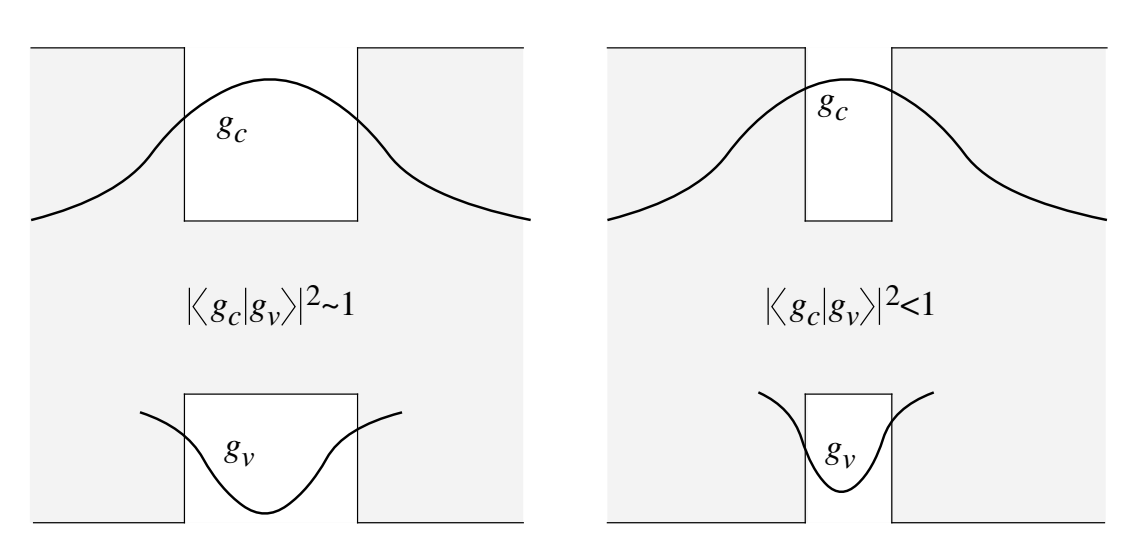
\includegraphics[width=\textwidth]{img/well_size.png}
		\\[0.5em]
		\refstepcounter{figure}
		\textbf{Figure~\thefigure.} Schematic showing how quantum well width affects electron and hole wavefunctions and their overlap integral. As the well becomes very narrow, the overlap between electron and hole wavefunctions decreases.
		\label{fig:well_size}
	\end{minipage}
\end{center}
In the context of quantum wells, the $1/W$ scaling of the absorption coefficient presents an interesting but potentially misleading aspect. This dependence originates from the assumption that the carrier wavefunctions are confined within a region of size comparable to the well width, $W$. According to this assumption, reducing the well width would indefinitely enhance the absorption coefficient. However, this conclusion is not entirely accurate.\\
When the quantum well becomes sufficiently narrow, the spatial extent of the electron and hole wavefunctions exceeds the well boundaries, meaning the carriers are no longer strictly confined to the well region. As a result, the spatial domain relevant for the electron wavefunction extends beyond $W$. Additionally, the discrepancy in effective mass between electrons and holes causes the electron wavefunction to spread more significantly, especially in wider wells. This leads to a reduced overlap between the electron and hole states, which in turn lowers the absorption coefficient from its idealized value of unity.\\
For typical semiconductor systems, an optimal well width is found to lie in the range of approximately 80–100~\AA, where the trade-off between confinement and wavefunction overlap yields the most effective absorption.

\section{Indirect Interband Transitions}
In certain semiconductors like Si, Ge, and AlAs—commonly referred to as indirect bandgap materials—optical transitions near the band edge require the participation of both photons and phonons to satisfy momentum conservation in $k$-space. Consequently, optical absorption in materials such as silicon and germanium is significantly weaker compared to that in direct bandgap materials like GaAs.\\
In a typical indirect interband transition, the process occurs through a second-order mechanism. Initially, the electron interacts with a photon and is excited to a virtual intermediate state within the direct band structure, maintaining momentum conservation. Subsequently, the electron is scattered into the indirect conduction band minimum through phonon interaction. Although momentum is conserved during this intermediate state, energy is not. This is because the intermediate step is a virtual process, where the energy mismatch is permissible due to the time–energy uncertainty principle, which relaxes strict energy conservation temporarily.\\
Ultimately, the entire two-step interaction does conserve energy. The transition probability is still governed by Fermi’s golden rule, albeit with a second-order perturbative matrix element. The expression for the transition rate is given by:
\begin{equation}
	W_{if} = \frac{2\pi}{\hbar} \int \left| \sum_n \frac{ \mel{f}{H_{\text{per}}}{n} \mel{n}{H_{\text{per}}}{i} }{E_i - E_n} \right|^2 \delta(E_f - E_i) \frac{d^3k}{(2\pi)^3}
\end{equation}
In the case of indirect transitions, the intermediate state is denoted by \( \ket{n} \), and the total perturbation is composed of the sum of the photon and phonon interactions:
\begin{equation}
	H_{\text{per}} = H_{\text{ph}} + H_{\text{ep}}
\end{equation}
Here, \( H_{\text{ph}} \) represents the electron-photon interaction, while \( H_{\text{ep}} \) corresponds to the electron-phonon interaction. Both can contribute to the transition rate. Among the two interaction paths, the photon-initiated processes typically dominate due to a smaller energy denominator (closer to the direct bandgap) compared to phonon-first processes, which involve larger energy gaps such as \( \abs{\vb{E}_{v\Gamma} - \vb{E}_{vX}} \) or \( \abs{\vb{E}_{v\Gamma} - \vb{E}_{vL}} \).\\
Accordingly, the scattering rate for a given \( \vb{k} \) is given by:
\begin{equation}
	W_{if}(\vb{k}) = \frac{2\pi}{\hbar} \int_f \left\{ \abs{M_{\text{em}}}^2 + \abs{M_{\text{abs}}}^2 \right\} \delta(E_f - E_i) \frac{d^3k}{(2\pi)^3}
\end{equation}
The matrix elements \( M_{\text{em}} \) and \( M_{\text{abs}} \) describe second-order interactions in which a photon is absorbed followed by either phonon emission or phonon absorption. Note that the photon energy \( \hbar \omega \) is smaller than the direct gap, so the intermediate state is virtual and energy conservation is not strictly required.\\
These second-order matrix elements take the form:
\begin{equation}
	\begin{aligned}
		M_{\text{abs}} & = \frac{ \left| \mel{c, \vb{k} + \vb{q}}{H_{\text{ep}}^{\text{abs}}}{c, \vb{k}} \right|^2 \left| \mel{c, \vb{k}}{H_{\text{ph}}^{\text{abs}}}{v, \vb{k}} \right|^2 }{(E_{g\Gamma} - \hbar \omega)^2} \\
		M_{\text{em}}  & = \frac{ \left| \mel{c, \vb{k} - \vb{q}}{H_{\text{ep}}^{\text{em}}}{c, \vb{k}} \right|^2 \left| \mel{c, \vb{k}}{H_{\text{ph}}^{\text{em}}}{v, \vb{k}} \right|^2 }{(E_{g\Gamma} - \hbar \omega)^2}
	\end{aligned}
\end{equation}
Phonon scattering arises mainly from optical intervalley phonons, with a deformation potential interaction described by:\\
\begin{equation}
	M_q^2 = \frac{\hbar D_{ij}^2}{2 \rho V \omega_{ij}} \left\{
	\begin{array}{ll}
		n(\omega_{ij})     & \text{(absorption)} \\
		n(\omega_{ij}) + 1 & \text{(emission)}
	\end{array}
	\right.
\end{equation}
Here, \( D_{ij} \) is the deformation potential constant, \( \rho \) is the material density, \( \omega_{ij} \) is the phonon frequency for the intervalley transition between the \(\Gamma\) point and the final valley, and \( V \) is the normalization volume. Because this is an indirect process, the overall transition probability is typically suppressed by a factor:
\begin{equation}
	\frac{M_q^2}{(E_{g\Gamma} - \hbar \omega)^2}
\end{equation}
This suppression factor is commonly in the range of \( 10^{-2} \) to \( 10^{-3} \), and exhibits a dependence on temperature via the phonon occupation number \( n(\omega_{ij}) \). Additionally, the indirect nature of the transition introduces a distribution of final states due to phonon scattering, and the rate must be integrated over all possible final states.\\
Thus, the total scattering rate becomes:
\begin{equation}
	\begin{aligned}
		W_{ij}(\vb{k}) & = \frac{2\pi}{\hbar} \frac{M_{\text{ph}}^2}{(E_{g\Gamma} - \hbar \omega)^2} \frac{\hbar D_{ij}^2}{2 \rho \omega_{ij}} J_\nu \\
		               & \times \left[ n(\omega_{ij}) N_c(E_1 + \hbar \omega_{ij}) + (n(\omega_{ij}) + 1) N_c(E_1 - \hbar \omega_{ij}) \right]
	\end{aligned}
\end{equation}
where \( J_\nu \) is the number of equivalent final valleys, \( N_c \) is the density of final states in the conduction band, and the energy \( E_1 \) is given by:
\begin{equation}
	E_1 = \hbar \omega - E_{gK'} - E_{\vb{k}}
\end{equation}
Here, \( E_{gK'} \) is the energy of the indirect bandgap, and \( E_{\vb{k}} \) is the initial kinetic energy of the electron measured from the valence band top.\\
To compute the total absorption coefficient, the rate \( W_{ij}(\vb{k}) \) must be summed over all initial states \( \vb{k} \) capable of absorbing a photon of energy \( \hbar \omega \). The integration limits for \( E_{\vb{k}} \) depend on whether a phonon is absorbed or emitted:
\begin{align*}
	E_{k,\text{max}} & = \hbar \omega - E_{gK'} + \hbar \omega_{ij} \quad \text{(phonon absorption)} \\
	E_{k,\text{max}} & = \hbar \omega - E_{gK'} - \hbar \omega_{ij} \quad \text{(phonon emission)}
\end{align*}
\begin{figure}[H]
	\centering
	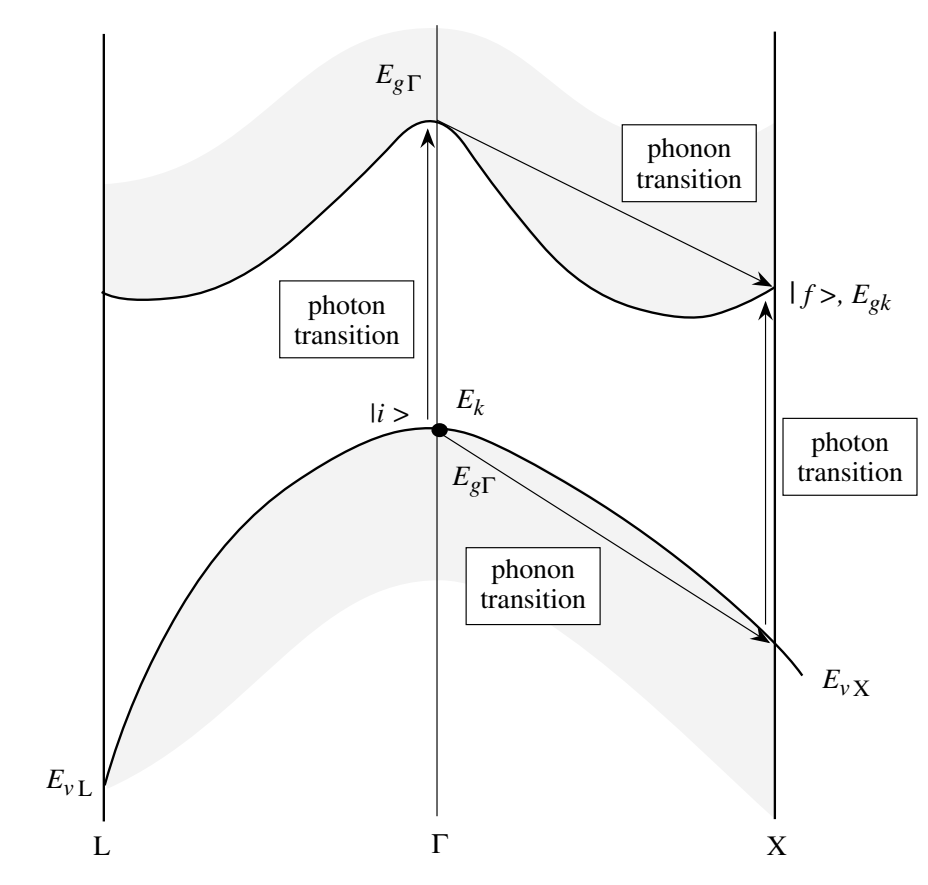
\includegraphics[width=0.6\textwidth]{img/phonon&photon.png}
	\caption{Two processes illustrating how an electron can transition from state $\lvert i \rangle$ to state $\lvert f \rangle$ through the combined action of a photon and a phonon. The photon energy does not need to match the vertical transition energy, as the intermediate state is virtual and not physically occupied by the electron.}
	\label{fig:indirect_transitions}
\end{figure}
To obtain the total transition rate, the quantity \( W(\vb{k}) \) is integrated over all initial valence states. Assuming a parabolic band structure, this becomes a straightforward integration over energy from 0 to \( E_{k,\text{max}} \), weighted by the density of initial states. For a single spin direction, the density of states in the valence band is given by \( N_v(E_{\vb{k}}) \), and we multiply the rate by \( 2V N_v(E_{\vb{k}}) \dd{E_{\vb{k}}} \). Performing the integration, we find the absorption rate for photons of energy \( \hbar \omega \) to be:
\begin{equation}
	\begin{aligned}
		W_{\text{abs}}(\hbar \omega) & = \frac{M_{\text{ph}}^2 D_{ij}^2 J_\nu (m_c m_v)^{3/2}}{8 \pi^2 (E_{g\Gamma} - \hbar \omega)^2 \hbar^6 \rho \omega_{ij}}                                                            \\
		                             & \times \left[ n(\omega_{ij}) \left( \hbar \omega - E_{gK'} + \hbar \omega_{ij} \right)^2 + (n(\omega_{ij}) + 1) \left( \hbar \omega - E_{gK'} - \hbar \omega_{ij} \right)^2 \right]
	\end{aligned}
\end{equation}
Here, \( M_{\text{ph}}^2 \) is the photon-related matrix element, expressed as:
\begin{equation}
	M_{\text{ph}}^2 = \frac{e^2 \hbar n_{\text{ph}}}{2 m_0^2 \epsilon \omega} \left| \vb{a} \cdot \vb{p}_{if} \right|^2
\end{equation}
The absorption coefficient \( \alpha \) is proportional to the transition rate divided by the photon flux, and is thus given by:
\[
	\alpha(\hbar \omega) = \frac{W_{\text{abs}}}{n_{\text{ph}} v_{\text{ph}}}
\]
Once the photon energy exceeds the absorption threshold, the coefficient begins to increase with energy as \( (\hbar \omega - E_{\text{th}})^2 \). This contrasts with direct transitions in direct-gap semiconductors, where the increase follows a \( (\hbar \omega - E_g)^{1/2} \) dependence.\\
In practical measurements, materials like silicon and germanium exhibit a much lower absorption coefficient near the band edge compared to direct-gap materials such as GaAs. However, once the photon energy surpasses the direct transition threshold, the absorption rises steeply due to the opening of direct transition channels.\\
It is important to note that in this formulation, only phonon-assisted absorption processes are considered. Nonetheless, other mechanisms—such as scattering by impurities, lattice defects, or alloy disorder—can also contribute to absorption in indirect semiconductors. Interestingly, materials with lower crystalline quality may sometimes show enhanced absorption compared to high-purity indirect semiconductors.\\
In amorphous materials such as amorphous silicon (a-Si), the absence of periodicity eliminates the need to conserve crystal momentum, since \( \vb{k} \) is no longer a good quantum number. This lack of \( \vb{k} \)-selection allows broader absorption, as transitions are not constrained by momentum conservation.


\section{Intraband Transitions}
Intraband optical transitions refer to electronic transitions that occur within the same energy band, either the conduction band or the valence band. In bulk semiconductors, these transitions cannot occur as first-order (i.e., single-photon or vertical) processes in momentum space due to the requirement for conservation of both energy and momentum. As a result, first-order intraband transitions are forbidden in bulk materials under normal conditions.\\
However, in quantum well systems, the situation differs significantly due to quantum confinement effects. The confinement leads to the formation of discrete energy levels or subbands within each band. Transitions between these subbands—referred to as inter-subband transitions—become allowed even though they still occur within the same main energy band.\\
These inter-subband transitions are a type of intraband process and are of particular interest in long-wavelength optoelectronic applications, such as in infrared detectors and quantum cascade lasers. The ability to engineer subband structures via quantum confinement makes quantum wells a valuable platform for exploiting such optical transitions.

\subsection{Intraband Transitions in Bulk Semiconductors}
In bulk semiconductors, intraband transitions require the involvement of a phonon or another scattering mechanism—such as ionized impurities, defects, or alloy disorder—to conserve momentum. These transitions are fundamentally second-order processes, analogous to those encountered in indirect interband absorption.\\
This type of absorption, often referred to as free carrier absorption, plays a crucial role in laser operation, especially because it contributes to optical losses in the cladding layers of the laser structure.\\
The behavior of free carrier absorption can be effectively modeled using the Drude theory of electrical transport. Under this framework, the incident optical field is treated as a time-varying electric field that causes conduction electrons to oscillate within the energy band. In the absence of scattering, these oscillations are lossless, resulting in no net energy absorption from the electromagnetic wave.\\
However, in real materials, various scattering mechanisms are always present. These interactions cause the electrons to dissipate part of the energy they absorb by emitting phonons, thus enabling net absorption of energy from the optical field. The frequency dependence of the absorption coefficient is then governed by:
\begin{equation}
	\alpha(\hbar \omega) \propto \frac{1}{\omega^2} \propto \frac{1}{\mu}
\end{equation}
where \( \omega \) is the angular frequency of the incident radiation, and \( \mu \) is the carrier mobility. This relationship indicates that the absorption decreases with increasing photon frequency and is also inversely proportional to the mobility. Hence, materials with high carrier mobility—where scattering is minimal—exhibit very low levels of free carrier absorption.


\subsection{Intraband Transitions in Quantum Wells}
Quantum well structures can significantly modify the electronic properties of semiconductors due to confinement effects. In such systems, the electronic wavefunctions are no longer plane waves along the growth (typically \( z \)) direction, allowing for intraband transitions that would otherwise be forbidden in bulk materials. These inter-subband transitions are enabled by quantum confinement and can be selectively accessed depending on the polarization of incident light.\\
Because the energy separation between subbands is highly sensitive to the well width, inter-subband transitions can be tuned for specific applications, especially in the far-infrared and terahertz spectral regions. This tunability makes quantum wells particularly valuable in detector technologies.\\
Consider a quantum well structure grown along the \( z \)-axis. Due to the confinement in this direction, the envelope wavefunctions for different subbands can be separated into transverse and longitudinal parts. For instance, the first two subband states can be written as:
\begin{equation}
	\begin{aligned}
		\psi^1(\vb{k}, z) & = g^1(z) e^{i \vb{k} \cdot \boldsymbol{\rho}} u^1_{n\vb{k}}(\vb{r}) \\
		\psi^2(\vb{k}, z) & = g^2(z) e^{i \vb{k} \cdot \boldsymbol{\rho}} u^2_{n\vb{k}}(\vb{r})
	\end{aligned}
\end{equation}
where \( g^1(z) \) and \( g^2(z) \) represent the envelope functions along the growth direction, \( \boldsymbol{\rho} \) is the in-plane coordinate, and \( u^i_{n\vb{k}}(\vb{r}) \) are the Bloch functions. These expressions reflect the separation of variables commonly used in effective mass approximations for quantum wells.\\
In analyzing optical transitions, especially vertical (in \( \vb{k} \)-space) ones, we observe that \( g^1 \) and \( g^2 \) are orthogonal. Furthermore, the central cell functions \( u^1 \) and \( u^2 \) are approximately identical for the different subbands, especially in the conduction band. Under this approximation, the matrix element for momentum transfer due to interaction with light becomes:
\begin{equation}
	\vb{p}_{if} = -\frac{i \hbar}{W} \int g^{2*}(z) e^{-i \vb{k} \cdot \boldsymbol{\rho}} \, \vb{a} \cdot \nabla g^1(z) e^{i \vb{k} \cdot \boldsymbol{\rho}} \, d^2 \rho \, dz
\end{equation}
Here, \( W \) is the width of the quantum well, and \( \vb{a} \) is the polarization vector of the incident light.\\
As in three-dimensional semiconductor systems, the momentum matrix element for inter-subband transitions vanishes if the light polarization vector (or the gradient operator in the integrand) lies within the in-plane \( \boldsymbol{\rho} \)-direction. For this reason, transitions involving \( x \)- or \( y \)-polarized light are forbidden due to symmetry, and the matrix element evaluates to zero. This holds unless strong band mixing exists, such as in valence band transitions, where the central cell functions may differ.\\
When light is polarized along the growth axis \( z \), the momentum matrix element for a transition between two subbands becomes:
\begin{equation}
	\vb{p}_{if} = -\frac{i\hbar}{W} \int g^{2*}(z) \, \hat{z} \, \frac{\partial}{\partial z} g^1(z) \, dz
\end{equation}
If the envelope functions \( g^1(z) \) and \( g^2(z) \) have even and odd parity, respectively, then the product \( g^2(z) \cdot \partial_z g^1(z) \) has overall odd parity, and the integral is non-zero. This configuration leads to a non-vanishing momentum matrix element under \( z \)-polarized excitation, which may be approximated as:
\begin{equation}
	\abs{\vb{p}_{if}} \approx \frac{\hbar}{W}
\end{equation}
This approximation remains valid as long as both the ground and excited states are well confined. If the excited state becomes delocalized, a more exact computation of the matrix element is required.
In the simple parabolic band approximation, the conduction subbands are assumed to be parallel, with an energy shift corresponding to the subband separation \( E_2 - E_1 \). Consequently, the joint density of states appears as a delta function at the transition energy. Incorporating Fermi-Dirac statistics, the absorption rate is given by:
\begin{equation}
	W_{\text{abs}} = \frac{\pi e^2 n_{\text{ph}}}{m_0^2 \omega \epsilon} \cdot \frac{1}{W} \sum_f \abs{\vb{p}_{if}}^2 \delta(E_2 - E_1 - \hbar \omega) f(E_1) \left[1 - f(E_2)\right]
\end{equation}
Assuming that the higher subband is initially unoccupied, the final-state occupation \( f(E_2) \) becomes zero, and the sum over final states reduces to:
\begin{equation}
	\sum_{\text{2nd subband}} \delta(E_2 - E_1 - \hbar \omega) f(E_1) = N_1
\end{equation}
where \( N_1 \) is the electron population in the first (lowest) subband.\\
The delta function implies an infinite absorption at resonance under the idealized parabolic band approximation. However, in realistic scenarios, this singularity is mitigated by nonparabolic effects and scattering mechanisms. Due to the finite lifetime of electron states, spectral broadening occurs, as dictated by the time–energy uncertainty principle.\\
If this broadening is modeled with a Gaussian profile, the two-dimensional density of states becomes:
\begin{equation}
	N(E) = \frac{N_1}{\sqrt{1.44 \pi} \sigma} \exp\left( -\frac{(E - E_{12})^2}{1.44 \sigma^2} \right)
\end{equation}
where \( E_{12} \) is the transition energy between subbands and \( \sigma \)  is the linewidth of the transition.
\begin{center}
	\begin{minipage}{0.65\textwidth}
		\centering
		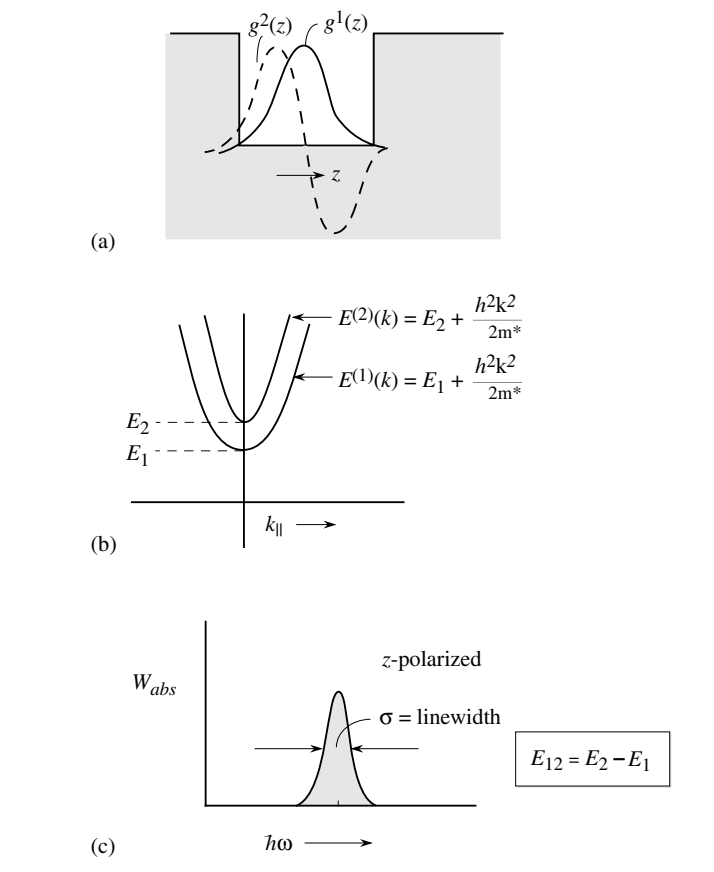
\includegraphics[width=\textwidth]{img/IntrabandTransitions.png}
		\\[0.5em]
		\refstepcounter{figure}
		\textbf{Figure~\thefigure.}Schematic illustration of:
		(a) envelope functions for two quantized energy levels in a quantum well,
		(b) the corresponding subband structure, and
		(c) the absorption spectrum for $z$-polarized light in the quantum well.
		\label{fig:IntrabandTransitions}
	\end{minipage}
\end{center}
The absorption coefficient increases rapidly as the quantum well width decreases. However, for very narrow wells, the assumption that electrons remain fully confined may no longer hold. For transitions with a linewidth of only 1–2 meV, the absorption coefficient can reach values on the order of $10^4$ cm$^{-1}$, making these transitions particularly attractive for use in photodetectors and optical modulators.\\
It is important to note that for $z$-polarized light in a quantum well with confinement along the $z$-direction, the light propagates in the plane of the substrate. As a result, vertical incidence does not lead to absorption. While valence band quantum wells exhibit band mixing that enables vertical light absorption, conduction band quantum wells lack this feature. This limitation can be problematic for photodetector applications. \\
To overcome this in imaging arrays, mirrors are often integrated into the detector structure to redirect vertically incident light so that it enters the device along the $x$-$y$ plane.


\section{Charge Injection and Radiative Recombination}
\subsection{Spontaneous Emission Rate}
When electrons and holes are injected into the conduction and valence bands of a semiconductor, they can recombine radiatively, resulting in photon emission. In the absence of photons already present in the optical cavity (i.e., when the photon density \( n_{\text{ph}} = 0 \)), this process corresponds to spontaneous emission. The characteristic spontaneous emission time in direct-gap materials is typically on the order of 0.5~ns, assuming both an electron and a hole occupy the same \( \vb{k} \)-state in their respective bands.\\
However, under realistic conditions, the actual recombination rate must account for the occupation probabilities of electrons and holes at each \( \vb{k} \)-point. Thus, one integrates over the full range of electronic states, weighted by the respective Fermi-Dirac distributions. The total spontaneous emission rate per unit volume (in cm\(^{-3}\)s\(^{-1}\)) is given by:
\begin{equation}
	R_{\text{spon}} = \frac{2}{3} \int d(\hbar \omega) \frac{2e^2 n_r \hbar \omega}{m_0^2 c^3 \hbar^2}
	\left[
		\int \frac{d^3 k}{(2\pi)^3} \abs{\vb{p}_{if}}^2
		\delta \left( E^e(\vb{k}) - E^h(\vb{k}) - \hbar \omega \right)
		f_e(E^e(\vb{k})) f_h(E^h(\vb{k}))
		\right]
\end{equation}
The outer integral over \( d(\hbar \omega) \) accounts for all photon energies, while the inner \( d^3k \) integral sums over momentum states. The prefactor \( 2/3 \) arises from averaging over random photon polarizations, assuming isotropic emission.\\
In quantum well structures, the formulation is adjusted to reflect the reduced dimensionality. Specifically, the three-dimensional density of states is replaced by the corresponding two-dimensional form. The spontaneous emission rate per unit area (in cm\(^{-2}\)s\(^{-1}\)) becomes:
\begin{equation}
	R_{\text{spon}} = \frac{2}{3} \int d(\hbar \omega) \frac{2e^2 n_r \hbar \omega}{m_0^2 c^3 \hbar^2}
	\sum_{n,m}
	\left[
		\int \frac{d^2 k}{(2\pi)^2} \abs{\vb{p}_{if}}^2
		\delta \left( E_n^e(\vb{k}) - E_m^h(\vb{k}) - \hbar \omega \right)
		f_e(E_n^e(\vb{k})) f_h(E_m^h(\vb{k}))
		\right]
\end{equation}
Here, \( n \) and \( m \) index the discrete electron and hole subbands in the quantum well.\\
Spontaneous emission is also commonly described in terms of the radiative lifetime \( \tau_o \), defined as the inverse of the spontaneous emission rate. Under this definition:
\begin{equation}
	R_{\text{spon}} = \frac{1}{\tau_o} \int d(\hbar \omega) N_{\text{cv}} \left\{ f^e(E^e) \right\} \left\{ f^h(E^h) \right\}
\end{equation}
In this expression, \( N_{\text{cv}} \) denotes the joint density of states for electron-hole recombination, and the integral represents the overlap of electron and hole occupation functions across energies matching the transition condition \( E^e - E^h = \hbar \omega \).
The spontaneous recombination rate plays a central role in both electronic and optoelectronic device performance. It is therefore useful to examine its behavior under a few common operating conditions. We focus here on electron-hole recombination under three distinct regimes:
\subsubsection*{i) Minority Carrier Injection}
When the electron density \( n \) is much greater than the hole density \( p \), and the semiconductor is heavily doped, we can assume that the occupation probability for electrons \( f^e(E^e) \approx 1 \). In this case, the recombination rate becomes dependent only on the hole distribution:
\begin{equation}
	R_{\text{spon}} \approx \frac{1}{\tau_o} \int d(\hbar \omega) N_{\text{cv}} f^h(E^h) \approx \frac{1}{\tau_o} \int d(\hbar \omega) N_h f^h(E^h) \left( \frac{m_r^*}{m_h^*} \right)^{3/2}
\end{equation}
This leads to:
\begin{equation}
	R_{\text{spon}} \approx \frac{1}{\tau_o} \left( \frac{m_r^*}{m_h^*} \right)^{3/2} p
\end{equation}
Thus, the spontaneous recombination rate is directly proportional to the minority carrier concentration (holes, in this case).
\subsubsection*{ii) Strong Injection}
Under conditions of high-level injection where both electrons and holes are introduced in significant numbers, the occupation probabilities \( f^e \) and \( f^h \) approach unity over the relevant energy range. Consequently, the recombination rate is limited by the lower of the two carrier densities:
\begin{equation}
	R_{\text{spon}} = \frac{n}{\tau_o} = \frac{p}{\tau_o}
\end{equation}
\subsubsection*{iii) Weak Injection}
In the low-injection regime, the Fermi-Dirac distributions can be approximated by Boltzmann statistics. In this case:
\begin{equation}
	f^e \cdot f^h \approx \exp\left( -\frac{E_c - E_{Fn}}{k_B T} \right)
	\exp\left( -\frac{E_{Fp} - E_v}{k_B T} \right)
	\exp\left( -\frac{\hbar \omega - E_g}{k_B T} \right)
\end{equation}
This leads to a modified recombination rate:
\begin{equation}
	R_{\text{spon}} = \frac{1}{2 \tau_o} \left( \frac{2\pi \hbar^2 m_r^*}{k_B T m_e^* m_h^*} \right)^{3/2} n p
\end{equation}
To account for excess carriers, we express total carrier densities as the sum of equilibrium and excess components:
\begin{equation}
	n = n_0 + \Delta n, \qquad p = p_0 + \Delta n
\end{equation}
Substituting into the recombination expression yields:
\begin{equation}
	R_{\text{spon}} \approx \frac{1}{2 \tau_o} \left( \frac{2\pi \hbar^2 m_r^*}{k_B T m_e^* m_h^*} \right)^{3/2}
	(\Delta n p_0 + \Delta n n_0)
\end{equation}
If we assume \( \Delta n = \Delta p \), we can define the recombination rate per excess carrier as:
\begin{equation}
	\frac{1}{\tau_r} = \frac{R_{\text{spon}}}{\Delta n} = \frac{1}{2 \tau_o}
	\left( \frac{2\pi \hbar^2 m_r^*}{k_B T m_e^* m_h^*} \right)^{3/2}
	(n_0 + p_0)
\end{equation}
At low levels of carrier injection, the recombination time \( \tau_r \) significantly exceeds the spontaneous emission lifetime \( \tau_o \). This occurs because, under such conditions, the probability that an electron finds a hole to recombine with is small.

\subsubsection*{iv) Inversion Condition}
A particularly relevant regime arises when the sum of the electron and hole occupation probabilities satisfies \( f^e + f^h = 1 \). This situation corresponds to population inversion, a critical condition in which emission and absorption processes occur with equal probability. Assuming symmetric carrier distributions with \( f^e \approx f^h = 1/2 \), the spontaneous recombination rate simplifies to:
\begin{equation}
	R_{\text{spon}} \approx \frac{n}{4 \tau_o} \approx \frac{p}{4 \tau_o}
\end{equation}
This leads to an effective radiative lifetime of approximately \( 4\tau_o \), which serves as a useful estimate when determining the threshold current of a semiconductor laser.\\
The gain and recombination dynamics explored here are fundamental to the design and analysis of both electronic and optoelectronic devices. From the above considerations, it becomes evident that the recombination lifetime associated with a single excess carrier can often be described by the general expression:
\begin{equation}
	\tau_r = \frac{\Delta n}{R_{\text{spon}}}
\end{equation}
In the cases of minority carrier injection or under strong injection conditions, \( \tau_r \approx \tau_o \). In general, the spontaneous recombination rate \( R_{\text{spon}} \) exhibits a strong dependence on carrier concentration, which in turn affects the recombination time \( \tau_r \).\\
Empirical measurements show that \( \tau_r \) can vary over several orders of magnitude depending on the injection level. For example, in gallium arsenide (GaAs), the radiative lifetime can range from microseconds at low injection to nanoseconds or less under high-injection conditions.


\subsection{Gain in a Semiconductor}
When both electrons and holes are injected into a semiconductor, as is the case in light-emitting devices, they may recombine radiatively, emitting photons. Under certain conditions, the rate of photon emission may exceed the rate of absorption, resulting in a net amplification of the optical field. This difference between stimulated emission and absorption defines the optical gain of the material.\\
In this regime, the gain is expressed as the difference between the emission coefficient and the absorption coefficient. A positive gain implies that a propagating optical wave will experience amplification rather than attenuation.\\
For parabolic energy bands, the gain as a function of photon energy \( \hbar \omega \) can be expressed as:
\begin{equation}
	g(\hbar \omega) = \frac{\pi e^2 \hbar}{n_r c m_0^2 \epsilon_0 (\hbar \omega)} \abs{\vb{a} \cdot \vb{p}_{if}}^2 N_{\text{cv}}(\hbar \omega)
	\left[ f^e(E^e) - \left(1 - f^h(E^h)\right) \right]
\end{equation}
This expression generalizes the form of the absorption coefficient by including the competition between emission and absorption processes. The square bracket term reflects the difference between the probability of photon emission, which is proportional to \( f^e \cdot f^h \), and that of photon absorption, proportional to \( (1 - f^e)(1 - f^h) \). When this difference is positive, the medium exhibits net optical gain.\\
The electron and hole energies are assumed to follow parabolic dispersions, such that:
\begin{equation}
	\hbar \omega - E_g = \frac{\hbar^2 k^2}{2 m_r^*}
\end{equation}
Here, \( E_g \) is the bandgap energy and \( m_r^* \) is the reduced effective mass. This relation provides the link between photon energy and the carrier wavevector \( k \) in the joint density of states.\\
The carrier energies in the conduction and valence bands are described using parabolic band approximations. For electrons and holes involved in optical transitions, the energies are given by:
\begin{equation}
	E^e = E_c + \frac{\hbar^2 k^2}{2 m_e^*} = E_c + \frac{m_r^*}{m_e^*}(\hbar \omega - E_g)
\end{equation}
\begin{equation}
	E^h = E_v - \frac{\hbar^2 k^2}{2 m_h^*} = E_v - \frac{m_r^*}{m_h^*}(\hbar \omega - E_g)
\end{equation}
In equilibrium, the carrier distribution is determined by the Fermi level \( E_F \). However, under injection conditions—such as in LEDs or semiconductor lasers—electrons and holes are injected into their respective bands, leading to the formation of quasi-Fermi levels \( E_{Fn} \) and \( E_{Fp} \).\\
At high injection levels, these quasi-Fermi levels may penetrate deep into the conduction and valence bands. When no electrons occupy the conduction band and no holes are present in the valence band (i.e., \( f^e(E^e) = 0 \) and \( f^h(E^h) = 0 \)), the material exhibits pure absorption, and the gain is simply the negative of the absorption coefficient: \( -\alpha(\hbar \omega) \).\\
A transition to optical gain occurs when the condition:
\begin{equation}
	f^e(E^e) > 1 - f^h(E^h)
\end{equation}
is satisfied. This regime corresponds to what is known as \textit{inversion}, where stimulated emission dominates over absorption.\\
In the presence of gain, the intensity of light traveling through the material increases exponentially with distance. This spatial dependence of optical intensity is described by:
\begin{equation}
	I(z) = I_0 \exp(g z)
\end{equation}
where \( I_0 \) is the initial intensity and \( g \) is the optical gain coefficient. This exponential growth contrasts with the usual case of absorption, where intensity decays as light propagates. The phenomenon of gain is the fundamental principle behind semiconductor laser operation.
\begin{center}
	\begin{minipage}{0.70\textwidth}
		\centering
		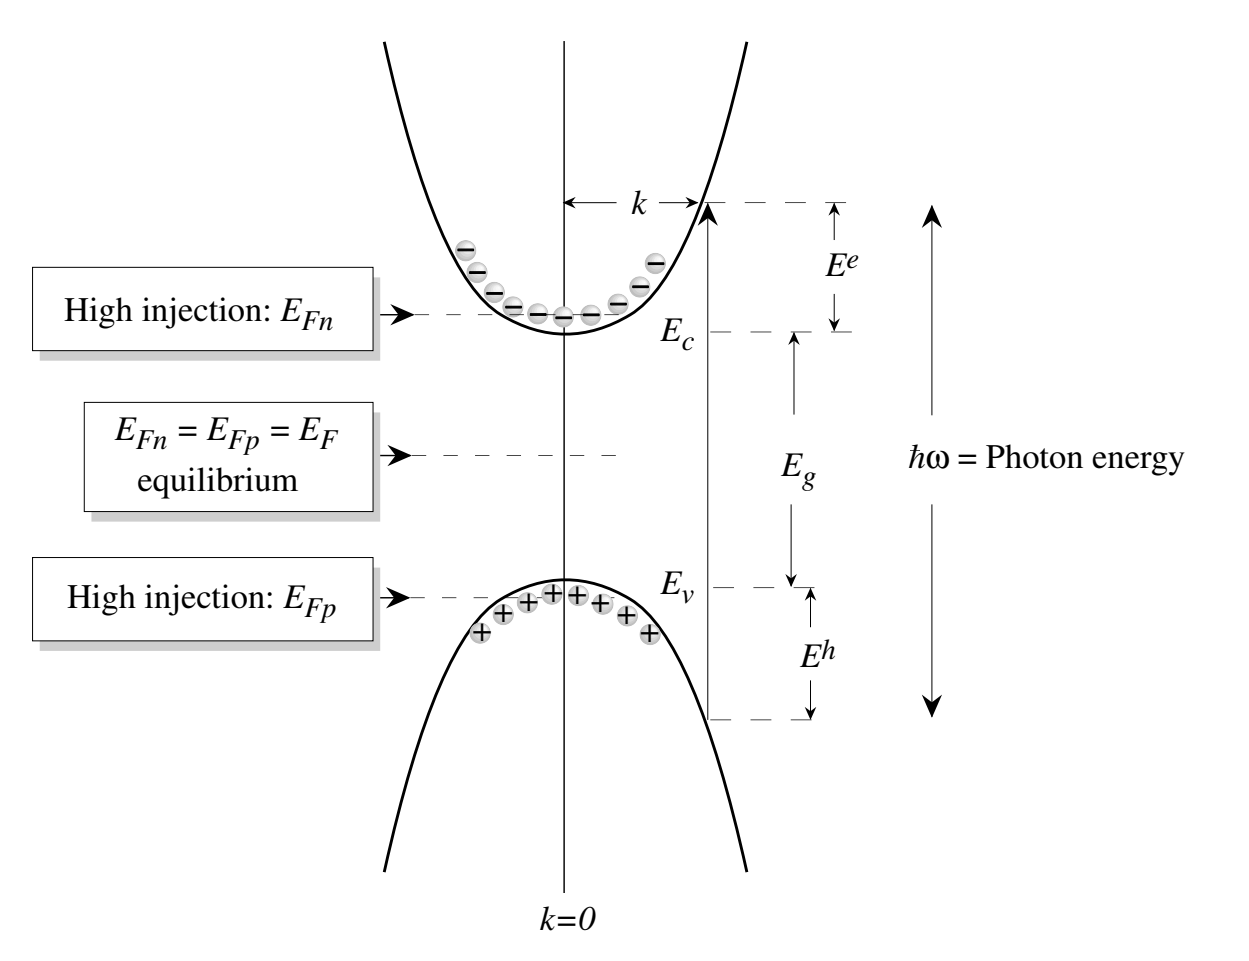
\includegraphics[width=\textwidth]{img/position_quasifermi.png}
		\\[0.5em]
		\refstepcounter{figure}
		\textbf{Figure~\thefigure.} Under high injection, the quasi-Fermi levels move deeper into the conduction and valence bands, indicating increased carrier densities. The optical behavior of the semiconductor is influenced by the carrier energies, which depend on the incident photon energy and the effective masses. These factors can lead to population inversion.
		\label{fig:position_quasifermi}
	\end{minipage}
\end{center}


\section{Nonradiative Recombination}
\subsection{Charge Injection: Nonradiative Effects}
In an ideal, defect-free semiconductor, Bloch's theorem dictates that electronic states exist only within the allowed energy bands, and no localized states are present within the bandgap. However, in real materials, defects and impurities—either intentional (e.g., dopants) or unintentional (e.g., vacancies or native defects)—introduce localized electronic states in the bandgap region. These states arise from chemical impurities or structural imperfections, leading to energy levels capable of capturing carriers.\\
While conduction and valence band states are spatially extended, defect-induced states are spatially localized and can act as traps. Electrons moving freely through the conduction band may become captured by such traps. Once trapped, these carriers may recombine with holes from the valence band without emitting a photon, resulting in a nonradiative recombination process. This mechanism competes with radiative recombination and becomes especially significant when defect density is high.\\
Let us consider a nonradiative recombination mechanism involving a midgap trap with density \( N_t \). If an empty trap is characterized by a capture cross-section \( \sigma \), and \( v_{\text{th}} \) is the thermal velocity of the carrier, then the average nonradiative lifetime for electrons and holes, denoted \( \tau_{nr}(e) \) and \( \tau_{nr}(p) \), are given by:
\begin{equation}
	\tau_{nr}(e) = \frac{1}{N_t v_{\text{th}} \sigma_n}, \qquad
	\tau_{nr}(p) = \frac{1}{N_t v_{\text{th}} \sigma_p}
\end{equation}
Here, \( \sigma_n \) and \( \sigma_p \) are the electron and hole capture cross-sections, respectively. These expressions form the basis of the Shockley-Read-Hall (SRH) theory of nonradiative recombination.
To simplify the treatment, we consider the following assumptions:
\begin{itemize}
	\item[i)] Equal lifetimes for electrons and holes: \( \tau_{nr}(e) = \tau_{nr}(p) = \tau_{nr} \),
	\item[ii)] The trap energy level \( E_t \) lies at midgap: \( E_t = E_{Fi} \),
	\item[iii)] High-injection condition: \( np \gg n_i^2 \), where \( n_i \) is the intrinsic carrier concentration.
\end{itemize}
Under these assumptions, the nonradiative recombination rate becomes:
\begin{equation}
	R_t = \frac{np}{\tau_{nr}(n + p)}
\end{equation}
This expression illustrates the dependence of the nonradiative recombination rate on both carrier densities and trap properties. It becomes especially relevant in materials with significant defect populations or under high-level injection conditions.
\begin{center}
	\begin{minipage}{0.80\textwidth}
		\centering
		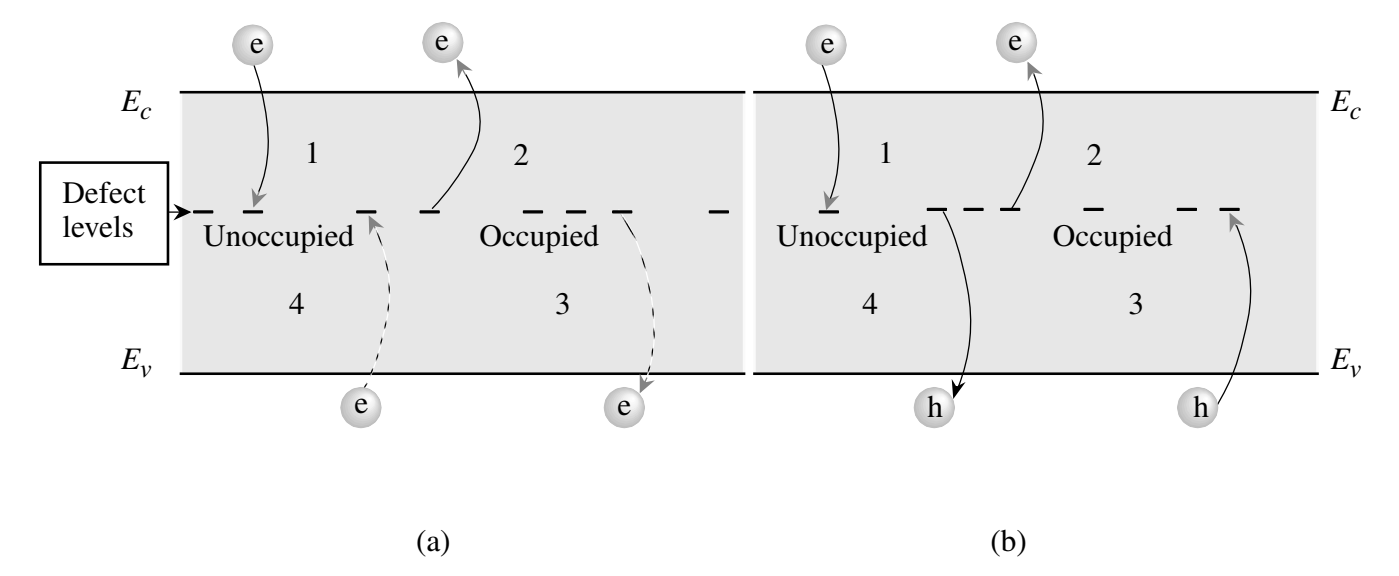
\includegraphics[width=\textwidth]{img/Recombination.png}
		\\[0.5em]
		\refstepcounter{figure}
		\textbf{Figure~\thefigure.} Illustration of trapping and recombination processes involving deep levels in the bandgap (dashed line).
		(a) Processes 1 and 2 depict electron trapping and emission, while 3 and 4 correspond to hole trapping and emission.
		(b) Electron-hole recombination via deep levels is also shown.
		\label{fig:Recombination}
	\end{minipage}
\end{center}

\section{Semiconductor Light Emitters}
Radiative recombination forms the physical foundation for semiconductor-based light-emitting devices such as light-emitting diodes (LEDs) and laser diodes (LDs). These devices are pivotal in modern technology, particularly in display systems and optical communication.\\
LEDs function through the mechanism of spontaneous emission, where electrons and holes recombine and emit photons randomly in phase and direction. In contrast, laser diodes rely on stimulated emission, a process that is contingent on the photon population already present in the active region of the device.\\
As previously described, stimulated emission occurs when an incoming photon induces an excited electron to recombine with a hole, emitting a new photon that is coherent with the stimulating one—i.e., it shares the same phase, frequency, and direction. This results in the generation of coherent light, which is the hallmark of laser operation.\\
In spontaneous emission, however, the photons emitted by electron-hole recombination events are incoherent, meaning they do not maintain a fixed phase relationship with each other. This fundamental difference between spontaneous and stimulated emission underpins the distinct optical characteristics of LEDs and LDs.\\
This section provides an overview of these two important device classes and the physical principles governing their operation.
\begin{center}
	\begin{minipage}{0.70\textwidth}
		\centering
		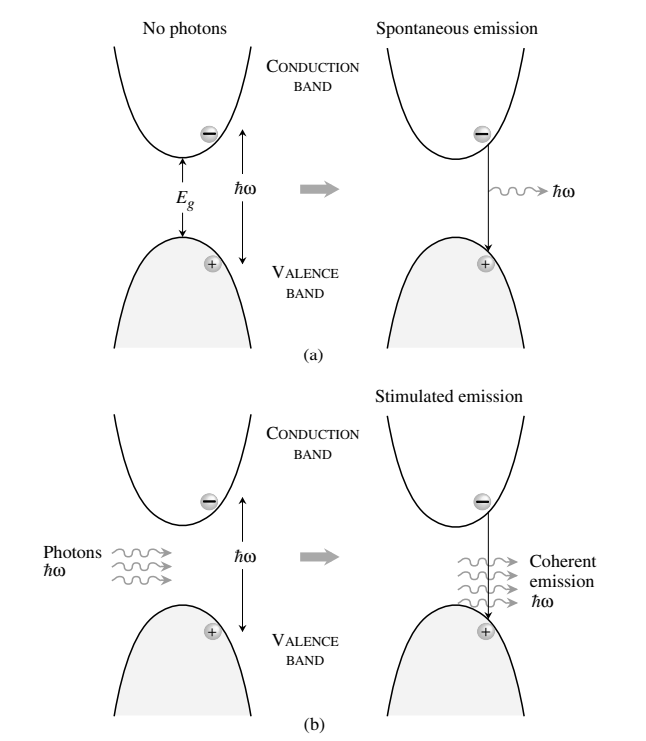
\includegraphics[width=\textwidth]{img/Spontaneus&Stimulated.png}
		\\[0.5em]
		\refstepcounter{figure}
		\textbf{Figure~\thefigure.} (a) Spontaneous emission: in the absence of external photons, electron-hole recombination generates photons with random phase.
		(b) Stimulated emission: in the presence of incident photons, recombination results in photons that are phase-coherent with the incoming ones.
		\label{fig:Spontaneus&Stimulated}
	\end{minipage}
\end{center}

\subsection{Light Emitting Diode}
The light-emitting diode (LED) operates as a forward-biased \( p\text{-}n \) junction diode. Under forward bias, minority carriers—electrons from the \( n \)-type side and holes from the \( p \)-type side—are injected across the junction. These carriers recombine in the active region, either radiatively, producing photons, or non-radiatively, dissipating energy as heat or via defects.\\
To optimize light output, the device must be engineered to maximize the probability of radiative recombination over non-radiative pathways. This is achieved by careful structural design and doping profiles.\\
During operation, electrons flow from the \( n \)-side into the \( p \)-side, while holes are injected from the \( p \)-side into the \( n \)-side. Ideally, recombination—and thus photon emission—should occur near the top surface of the device. Emission deep within the structure is undesirable, as photons generated in these regions have a higher likelihood of being reabsorbed before escaping.\\
To mitigate this issue, LEDs are typically designed so that the top layer is \( p \)-type. In such configurations, electrons (the majority carriers in the \( n \)-type material) dominate the injection current. Since radiative efficiency is enhanced when electron injection dominates, the diode is fabricated with asymmetric doping—heavily doped on the \( p \)-side and more lightly doped on the \( n \)-side. This ensures that most of the recombination and subsequent light emission occurs close to the emitting surface, improving external quantum efficiency.
\begin{center}
	\begin{minipage}{0.90\textwidth}
		\centering
		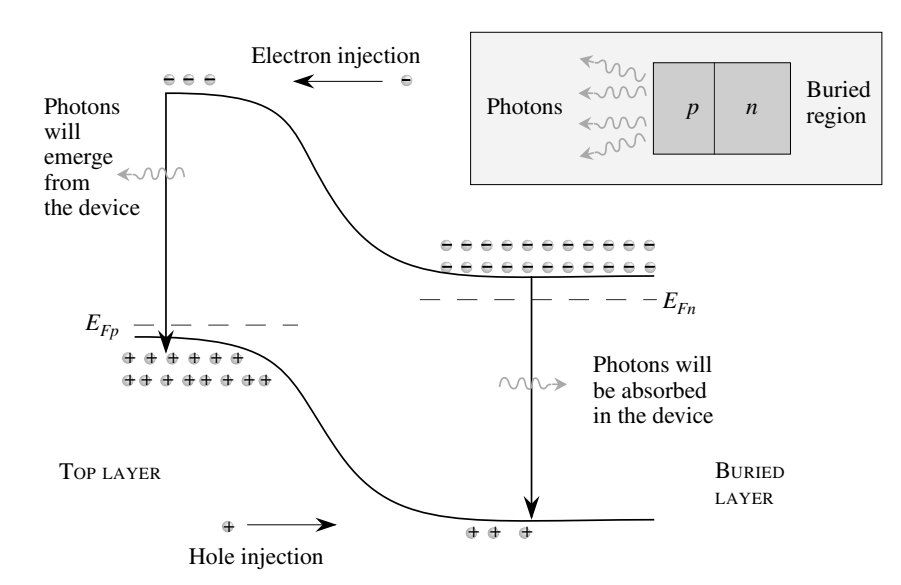
\includegraphics[width=\textwidth]{img/LED.png}
		\\[0.5em]
		\refstepcounter{figure}
		\textbf{Figure~\thefigure.} In a forward-biased p–n junction, both electrons and holes are injected across the junction. Holes injected into the buried $n$-region generate photons deep within the device, which are unlikely to escape. In contrast, electrons injected into the $p$-region recombine near the surface, producing photons with a higher probability of emerging from the LED.
		\label{fig:LED}
	\end{minipage}
\end{center}

\subsection{Laser Diode}
The laser diode, like the LED, relies on a forward-biased \( p\text{-}n \) junction to inject electrons and holes into the active region. However, unlike LEDs, laser diodes are engineered to incorporate an optical cavity that confines and guides the generated photons.\\
This optical cavity functions as a resonator, allowing photons to reflect back and forth multiple times. Because only a fraction of the emitted photons escapes the cavity during each round-trip, the internal photon density increases, enabling the conditions necessary for stimulated emission and optical amplification.\\
A commonly employed resonant structure in semiconductor lasers is the Fabry-Pérot cavity. This cavity typically consists of two parallel reflective surfaces—often cleaved crystal facets or deposited mirrors—that define the longitudinal boundary of the laser. These reflective interfaces ensure that only specific optical wavelengths form standing wave patterns, or resonant modes, within the cavity.\\
The condition for resonance requires that the cavity length \( L \) accommodate an integer number of half-wavelengths of the light, given by:
\begin{equation}
	L = \frac{q \lambda}{2}
\end{equation}
where \( q \) is an integer, and \( \lambda \) is the wavelength of light inside the semiconductor material. The wavelength \( \lambda \) within the material is related to the free-space wavelength \( \lambda_0 \) by the refractive index \( n_r \) of the cavity medium:
\begin{equation}
	\lambda = \frac{\lambda_0}{n_r}
\end{equation}
In practice, the Fabry-Pérot cavity includes two polished and reflective facets on opposite ends of the diode structure, which reflect most of the light back into the cavity. The remaining surfaces are often intentionally roughened or coated to prevent unwanted reflections, ensuring directional emission and suppressing lateral modes.\\
This resonant structure allows the laser diode to support coherent light emission by sustaining specific longitudinal modes, which meet the resonance condition. The combination of carrier injection, optical feedback, and gain results in the lasing action that defines the operation of semiconductor lasers.\\
When a planar heterostructure is employed to confine the optical mode in the \( z \)-direction, the governing equation for the optical field becomes:
\begin{equation}
	\frac{d^2 F_k(z)}{dz^2} + \left( \frac{\epsilon(z) \omega^2}{c^2} - k^2 \right) F_k(z) = 0
\end{equation}
In this expression, \( F \) represents the electric field associated with the optical wave, \( \epsilon(z) \) is the spatially varying dielectric constant, and \( k \) is the transverse wavevector. The spatial variation of \( \epsilon(z) \) is engineered to confine the optical mode along the \( z \)-axis. This confinement is typically achieved by embedding the active region within cladding layers made of materials with a larger bandgap.\\
A critical figure of merit for such a laser structure is the optical confinement factor \( \Gamma \), which quantifies the fraction of the optical field energy residing in the active region where electron-hole recombination and photon generation occur. It is defined as:
\begin{equation}
	\Gamma = \frac{\int_{\text{active region}} |F(z)|^2 dz}{\int |F(z)|^2 dz}
\end{equation}
In conventional double-heterostructure lasers based on bulk materials, the confinement factor \( \Gamma \) approaches unity when the active region thickness is on the order of \( \sim 1 \, \mu\text{m} \). However, in advanced quantum well laser designs, \( \Gamma \) can be as low as 1\%. Despite this reduced confinement, quantum well lasers often outperform bulk devices due to their enhanced electronic properties, such as a higher density of states arising from the two-dimensional nature of quantum wells.
\begin{center}
	\begin{minipage}{0.90\textwidth}
		\centering
		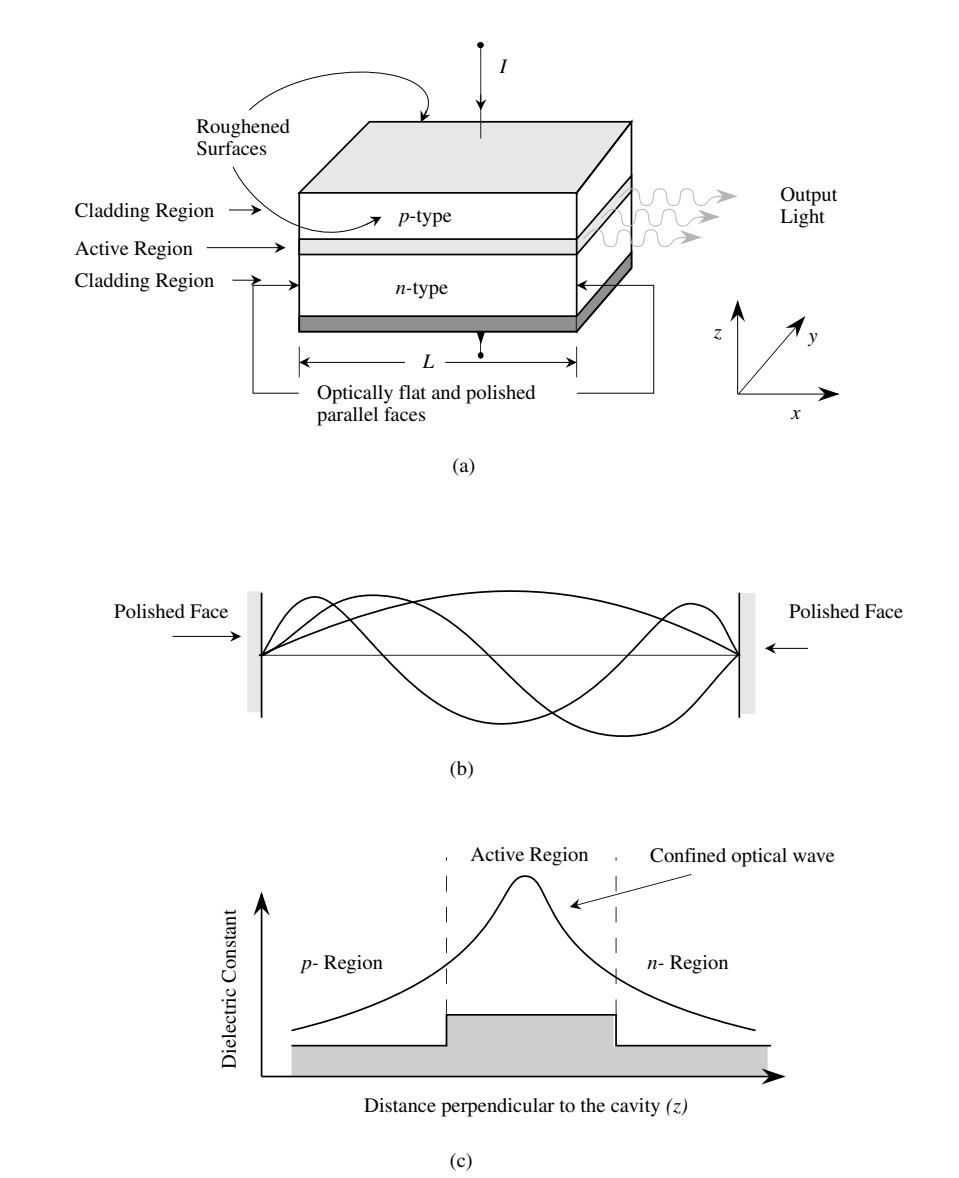
\includegraphics[width=\textwidth]{img/Laser.png}
		\\[0.5em]
		\refstepcounter{figure}
		\textbf{Figure~\thefigure.} (a) Schematic of a laser structure showing the optical cavity and mirrors that confine photons. The active region may be a simple double heterostructure or a more complex quantum well design.
		(b) Stationary cavity modes, established by the mirror-induced resonances.
		(c) Optical confinement resulting from spatial variations in the dielectric constant.
		\label{fig:Laser}
	\end{minipage}
\end{center}

\subsubsection{Optical Absorption, Loss and Gain}
When excess carriers are injected into the active region of a semiconductor laser—either by forward biasing a \( p\text{-}n \) junction or through optical pumping—the optical gain in the medium transitions from negative to positive over a certain energy range. This behavior is typically illustrated in gain versus injection current plots.\\
The net optical gain is generated solely within the active region where electron-hole recombination occurs. This region is often extremely thin, especially in quantum well lasers. For such structures, the relevant parameter is the \textit{cavity gain}, defined as:
\begin{equation}
	\text{Cavity gain} = g(\hbar \omega) \, \Gamma
\end{equation}
where \( g(\hbar \omega) \) is the material gain as a function of photon energy, and \( \Gamma \) is the optical confinement factor, which represents the fraction of the optical field overlapping with the gain region.\\
In double heterostructure lasers based on bulk semiconductors, \( \Gamma \) is typically close to unity. In contrast, in quantum well lasers, \( \Gamma \) may be as low as 0.01 due to the extremely thin active region. Nevertheless, quantum well lasers can achieve substantial cavity gain because the material gain \( g \) in such structures is significantly enhanced for a given injection level, owing to their two-dimensional carrier confinement.\\
For laser action to begin, the cavity gain must exceed the optical losses in the system. These losses, often grouped under the term \( \alpha_{\text{loss}} \), arise from two primary sources:
\begin{itemize}
	\item[i)] Absorption of photons in passive regions of the structure, such as the cladding layers and electrical contacts;
	\item[ii)] Photon escape losses at the output facets of the cavity.
\end{itemize}
The dominant contribution to \( \alpha_{\text{loss}} \) typically comes from free carrier absorption, which is a second-order interaction involving mobile charge carriers. In high-purity materials with minimal doping and low defect density, this loss can be as low as \( 10 \, \text{cm}^{-1} \). It is important to note that cavity loss is sensitive to both the level of doping and the quality of the crystal structure.
Another significant source of photon loss arises from the escape of photons through the cavity mirrors. This form of loss is termed the \textit{cavity loss}, and it is expressed as:
\begin{equation}
	\alpha_{\text{cavity}} = -\frac{1}{L} \ln R
\end{equation}
where \( L \) is the cavity length, and \( R \) is the reflectivity of the mirror surfaces defining the resonant cavity.
In the case of a semiconductor-air interface, the reflectivity \( R \) can be approximated by the Fresnel formula:
\begin{equation}
	R = \left( \frac{n_r - 1}{n_r + 1} \right)^2
\end{equation}
where \( n_r \) is the refractive index of the semiconductor material.
It follows that minimizing optical loss requires maximizing the reflectivity \( R \), which can be achieved using high-quality dielectric coatings or Bragg reflectors. Moreover, since the loss depends logarithmically on \( R \), even small increases in reflectivity can lead to substantial reductions in \( \alpha_{\text{cavity}} \). This makes mirror design a critical factor in the efficiency of laser diodes, particularly in applications demanding low threshold currents and high output power.

\subsubsection{Laser Below and Above Threshold}
In this section, we analyze the light output as a function of injected current density in a laser diode. This corresponds to the light output in the lasing mode. When compared with an LED, there is a key difference: the laser diode exhibits an abrupt change in light output behavior around a specific threshold condition. This threshold condition occurs when the cavity gain overcomes the cavity loss for some photon energy, defined as
\begin{equation}
	\Gamma g(\hbar\omega) = \alpha_{\text{loss}} - \frac{\ln R}{L}
\end{equation}
In high-quality lasers, \( \alpha_{\text{loss}} \sim 10~\text{cm}^{-1} \), and reflection losses may contribute a similar amount. Another useful definition in laser operation is the condition of transparency, which occurs when the optical gain is zero:
\begin{equation}
	\Gamma g(\hbar\omega) = 0
\end{equation}
Under forward bias, electrons and holes are injected into the active region, where they recombine and emit photons. Initially, at low injection levels, the number of carriers is insufficient to produce significant gain, and emitted photons are either absorbed or lost. As the bias increases, carrier injection increases until the gain reaches the threshold needed to balance the losses, allowing photon buildup in the cavity. Beyond this threshold, stimulated emission dominates spontaneous emission, resulting in a sharp increase in light output.\\
Let \( n_{th} \) be the carrier density at threshold. Then the threshold current density due to radiative recombination is given by
\begin{equation}
	J_r(th) = \frac{e n_{th} d_{\text{las}}}{\tau_r} = \frac{e n_{th}(2D)}{\tau_r}
\end{equation}
\begin{center}
	\begin{minipage}{0.80\textwidth}
		\centering
		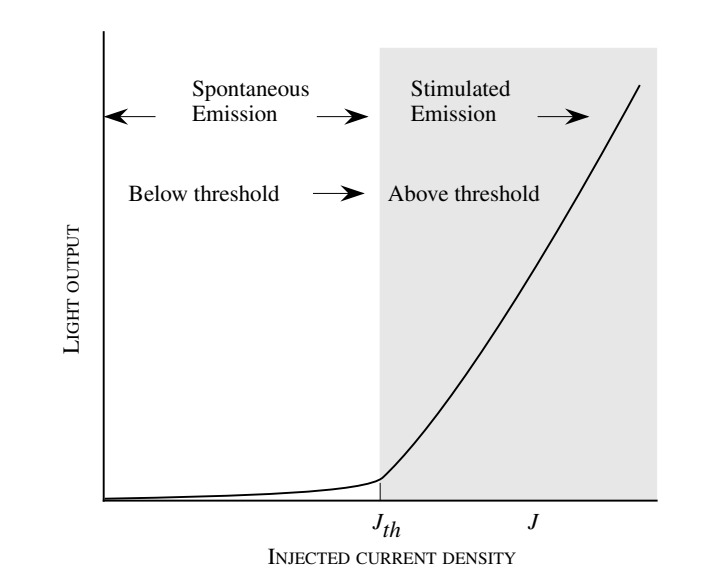
\includegraphics[width=\textwidth]{img/J_Thr.png}
		\\[0.5em]
		\refstepcounter{figure}
		\textbf{Figure~\thefigure.}
		\label{fig:J_Thr}
	\end{minipage}
\end{center}
where \( d_{\text{las}} \) is the thickness of the active region and \( n(2D) \) is the areal carrier density.
The radiative lifetime is \( \tau_r \), which under lasing conditions is given by:
\begin{equation}
	\tau_r \sim \frac{\tau_0}{4}
\end{equation}
In addition to the radiative current, we also have a non-radiative current \( J_{nr} \). For Auger processes, we have:
\begin{equation}
	J_{nr} = e F n^3 d_{\text{las}}
\end{equation}
The total threshold current density is then:
\begin{equation}
	J_{th} = \frac{e n_{th}(2D)}{\tau_r} + e F n_{th}^3 d_{\text{las}}
\end{equation}
\begin{center}
	\begin{minipage}{0.90\textwidth}
		\centering
		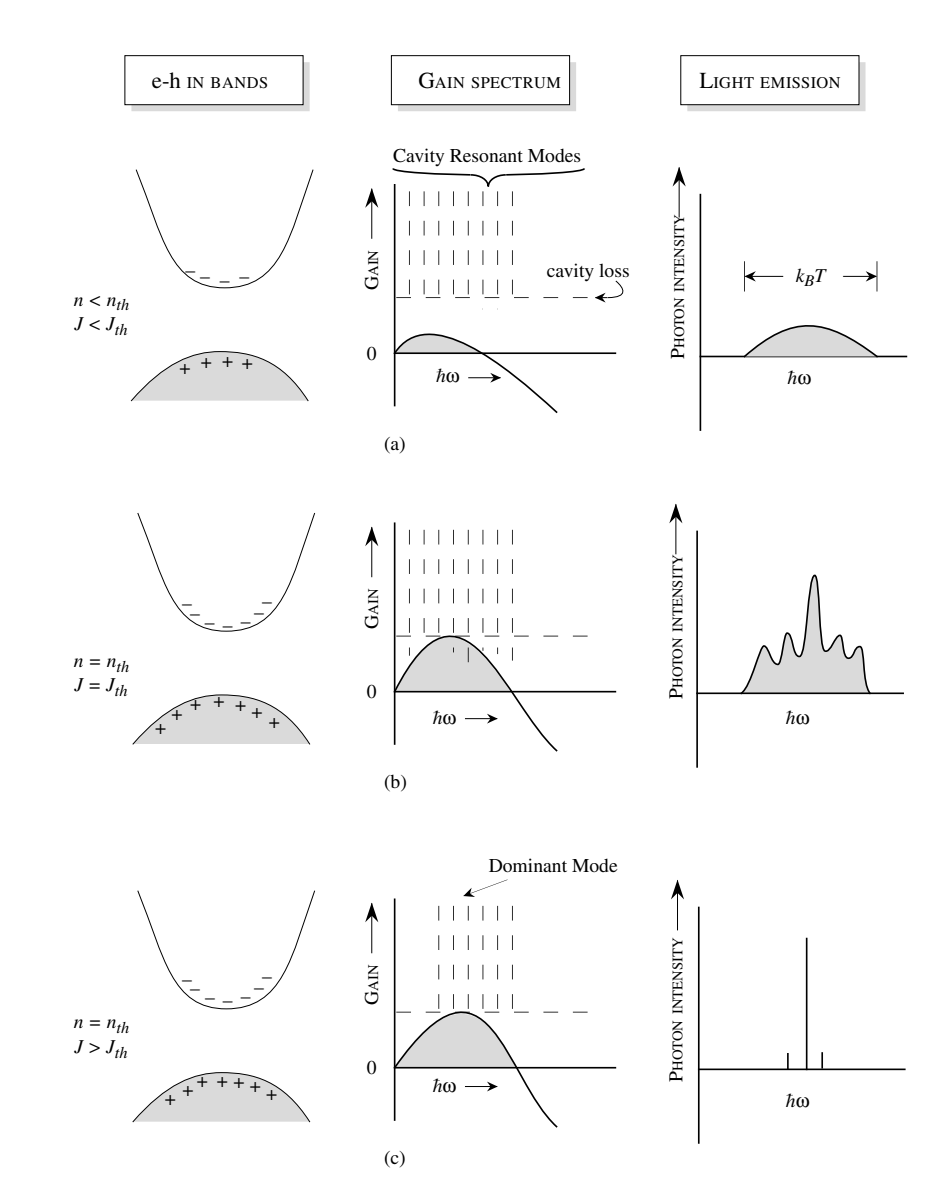
\includegraphics[width=\textwidth]{img/Laser_Threshold.png}
		\\[0.5em]
		\refstepcounter{figure}
		\textbf{Figure~\thefigure.} (a) Laser operating below threshold: gain is insufficient to overcome cavity losses, and emission is broad, similar to an LED.
		(b) At threshold: a few resonant modes begin to dominate the emission spectrum.
		(c) Above threshold: the gain spectrum remains unchanged, but stimulated emission causes a single mode to dominate the output.
		\label{fig:Laser_threshold}
	\end{minipage}
\end{center}
